% Emacs settings: -*-mode: latex; TeX-master: "manual.tex"; -*-

\chapter{Running \MCS}
\label{c:running}


%FIXME DESCRIBE NEW Python TOOLS!!

This chapter describes usage of the McStas simulation package. 
In case of problems regarding installation or usage, the McStas mailing
list~\cite{mcstas_webpage} or the authors should be contacted.

\index{McStas!structure}
Performing a simulation using \MCS can be divided into the following
steps/elements
\begin{itemize}
\item{The structure of \MCS is illustrated in
    Figure~\ref{fig:structure}.}
\item{To use \MCS, an instrument
definition file describing the instrument to be simulated must be
written. Alternatively, an example instrument file can be obtained
from the \verb+examples/+ directory in the distribution or from
another source.}
\item{The input files (instrument and component files) are written in the \MCS
meta-language and are edited either by using your favorite editor
or by using the built-in editor of the graphical user interface
(\texttt{mcgui}).}
\item{Next, the instrument and component files are compiled using the \MCS
compiler, relying on built-in features from the FLEX and Bison facilities to produce a C program.}
\item{The resulting C program can then be
compiled with a C compiler and run in combination with various
front-end programs for example to present the intensity at the
detector as a motor position is varied.}
\item{The output data may be analyzed and visualized in the same way as regular
    experiments by using the data handling and visualization tools in \MCS
    based on Perl/Python in combination with \verb+chaco+, \verb+matplotlib+,
    Matlab, GNUPlot or PGPLOT. Further data output formats including NeXus
    are available, see section \ref{s:analyze}.\index{Tools}}
\end{itemize}


\begin{figure}[pt!]
\begin{center}
    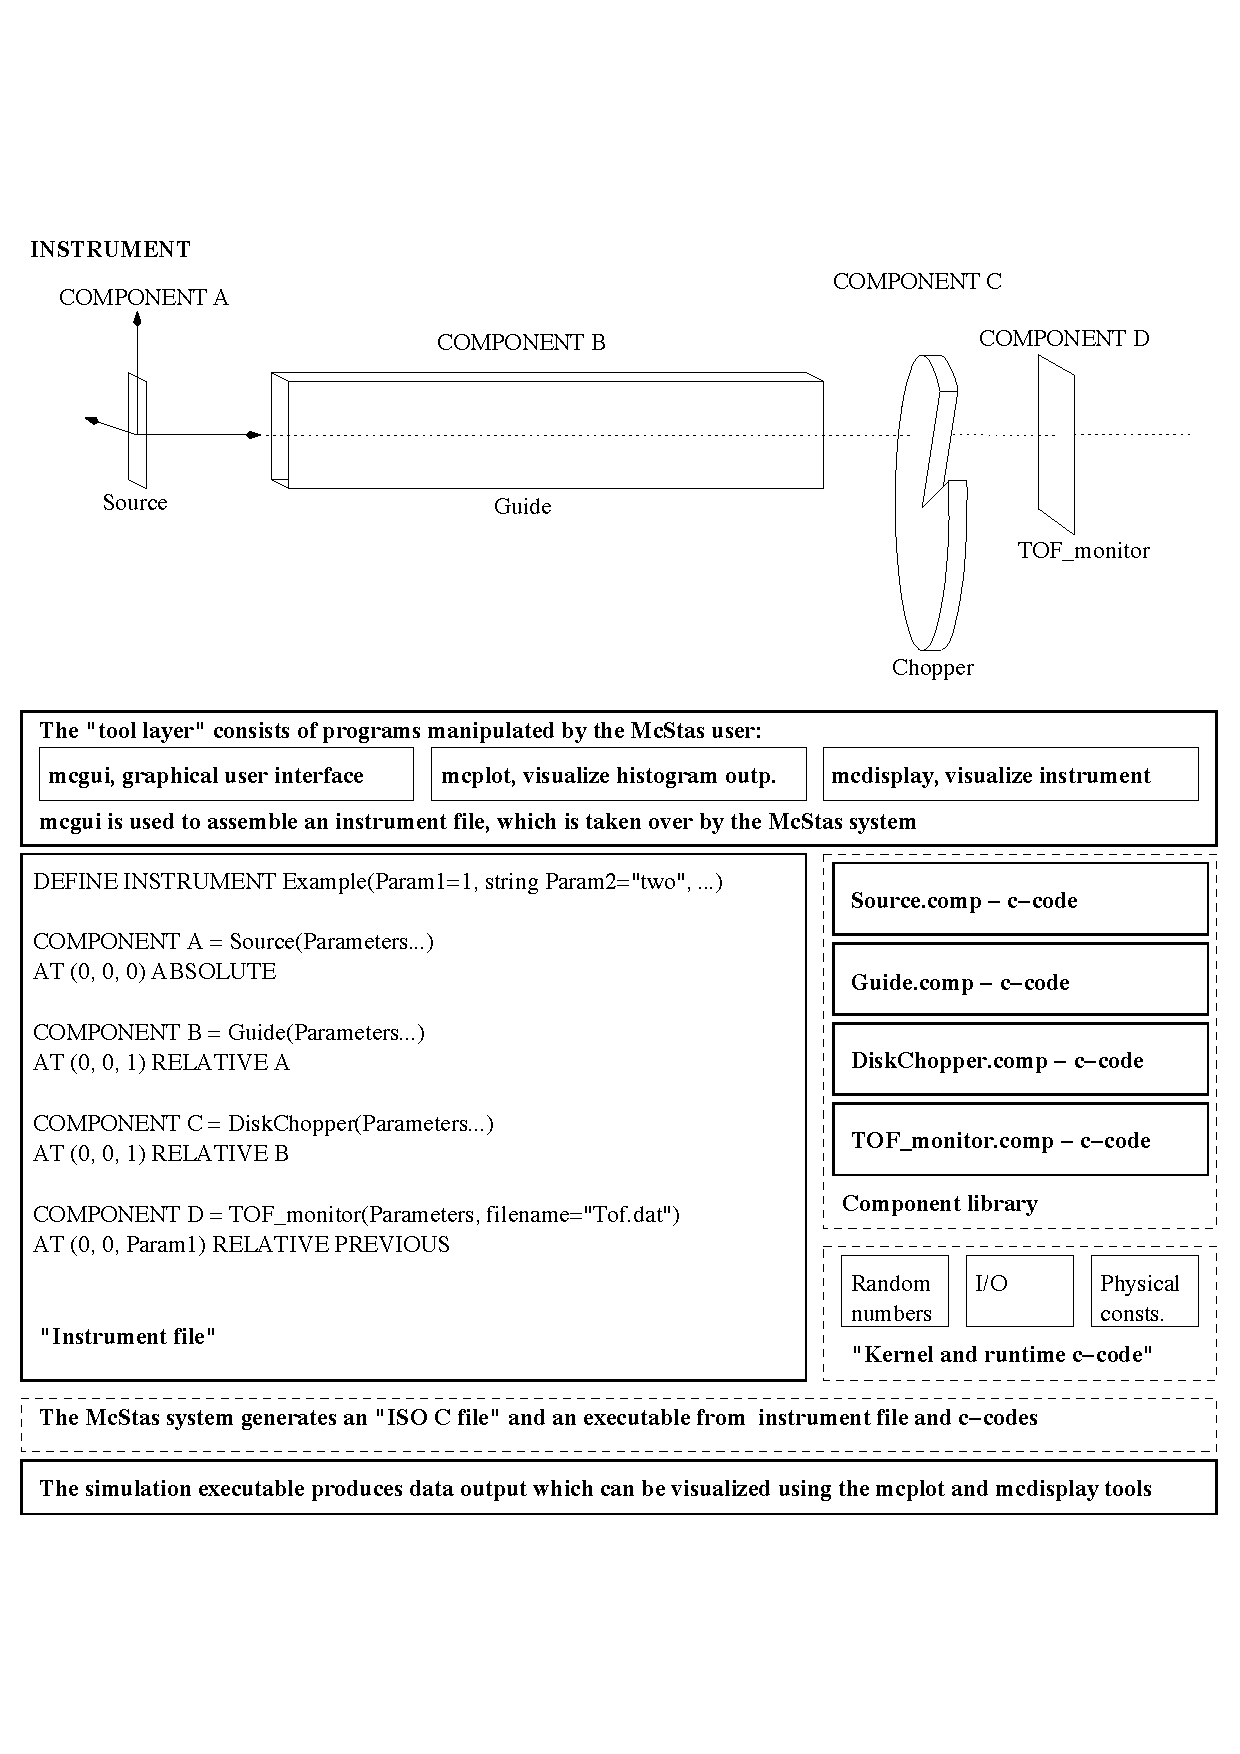
\includegraphics[width=\textwidth]{figures/mcstas_software.pdf}
\end{center}
\caption{An illustration of the structure of \MCS.\index{McStas!structure}}
\label{fig:structure}
\end{figure}

%%%%%%%%%%%%%%%%%%%%%%%%%%%%%%%%%%%%%%%%%%%%%%%%%%%%%%%%%%%%%%%%%%%%%%%%%%%%%%%%
\section{Installation and updates}
\label{s:install}

\index{McStas!installation}
\index{Installation}
For installation notes, see the web site~\cite{mcstas_webpage}.
In case of problems, write the support mailing list,
or contact the authors.

%-------------------------------------------------------------------------------
\subsection{Important note for Windows users} 
\index{Microsoft Windows|see{Windows}}
\index{MS Windows|see{Windows}}
\index{Windows!file and directory names with spaces}
\index{Windows!Perl distribution}
\index{Perl!ActiveState for Windows}
It is a known problem that some of
the \MCS tools do not support filenames / directories with spaces.
We are working on a more general approach to this problem, which will
hopefully be solved in a further release. We recommend to use
ActiveState \textbf{Perl 5.10}. (Note that as of \MCS 1.10, all needed
support tools for Windows are bundled with \MCS in a single installer file.)

%-------------------------------------------------------------------------------
\subsection{New releases of \MCS}
\index{McStas!release scheme}
\index{Release scheme}

Releases of new versions of a software package can today be carried out more or
less continuously. However, users do not update their software on a daily basis,
and as a compromise we have adopted the following policy of \MCS .

\begin{itemize}
\item The versions {\version}.x will possibly contain bug fixes and minor new
  functionality. A new manual will, however, not be released and the
  modifications are documented on the \MCS web-page. The extensions of the
  forthcoming version {\version}.x are also listed on the web, and new versions
  may be released quite frequently when it is requested by the user community.
\end{itemize}

%%%%%%%%%%%%%%%%%%%%%%%%%%%%%%%%%%%%%%%%%%%%%%%%%%%%%%%%%%%%%%%%%%%%%%%%%%%%%%%%
\section{Brief introduction to the graphical user interface}
\label{s:brief}

\index{McStas!running through the GUI|(}
\index{Graphical User Interface|see{mcgui}}
\index{GUI|see{mcgui}}
\indexTOOL{mcgui|(textbf}

This section gives an ultra-brief overview of how to use \MCS once it
has been properly installed. It is intended for those who do not read
manuals if they can avoid it. For details on the different steps, see
the following sections. This section uses the
\verb+Samples_vanadium.instr+ file supplied in the \verb+examples/+
directory of the \MCS distribution. %, see appendix~\ref{a:Samples_vanadium.instr}.

To start the graphical user interface of McStas, run the
\verb+mcgui+ command which will open a window
with a number of menus,
see figure~\ref{fig:mcgui}. 
\begin{figure}[htb!]
  \begin{center}
    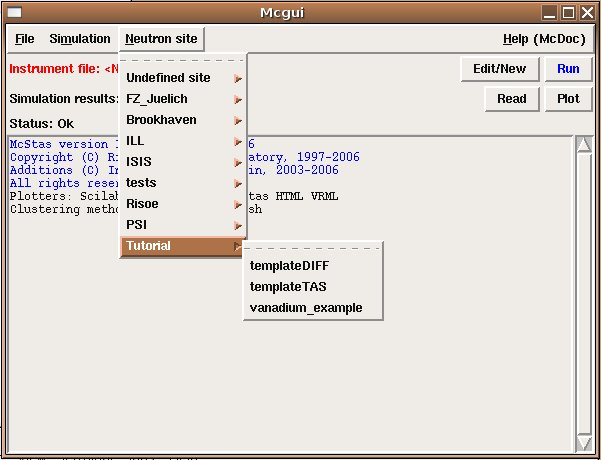
\includegraphics[width=0.55\textwidth]{figures/mcgui}
  \end{center}
\caption{The graphical user interface \texttt{mcgui}.}
\label{fig:mcgui}
\end{figure}
\label{p:neutronsite}
To load an instrument, select ``Tutorial'' from the ``Neutron site''
menu and open the file \verb+Samples_vanadium+. Next, check that the current plotting backend setting
(select ``Choose backend'' from the ``Simulation'' menu) corresponds
to your system setup.
\begin{itemize}
\item{by editing
the \verb+tools/perl/mcstas_config.perl+ setup file of your
installation}
\item{by setting the \verb+MCSTAS_FORMAT+ environment
variable.}
\end{itemize}
\indexEV{MCSTAS\_FORMAT}

Next, select ``Run simulation'' from the ``Simulation'' menu.
McStas will translate the definition into an executable program and pop
up a dialog window. Type a value for the ``ROT'' parameter ({\em e.g.}
90), check the ``Plot results'' option, and select ``Start''. The
simulation will run, and when it finishes after a while the results will
be plotted in a window. Depending on your chosen plotting backend, the
presented graphics will resemble one of those shown in figure
\ref{fig:mcplot_figs}.\indexTOOL{mcplot}
\begin{figure}[htb!]
    \begin{minipage}{.45\textwidth}
    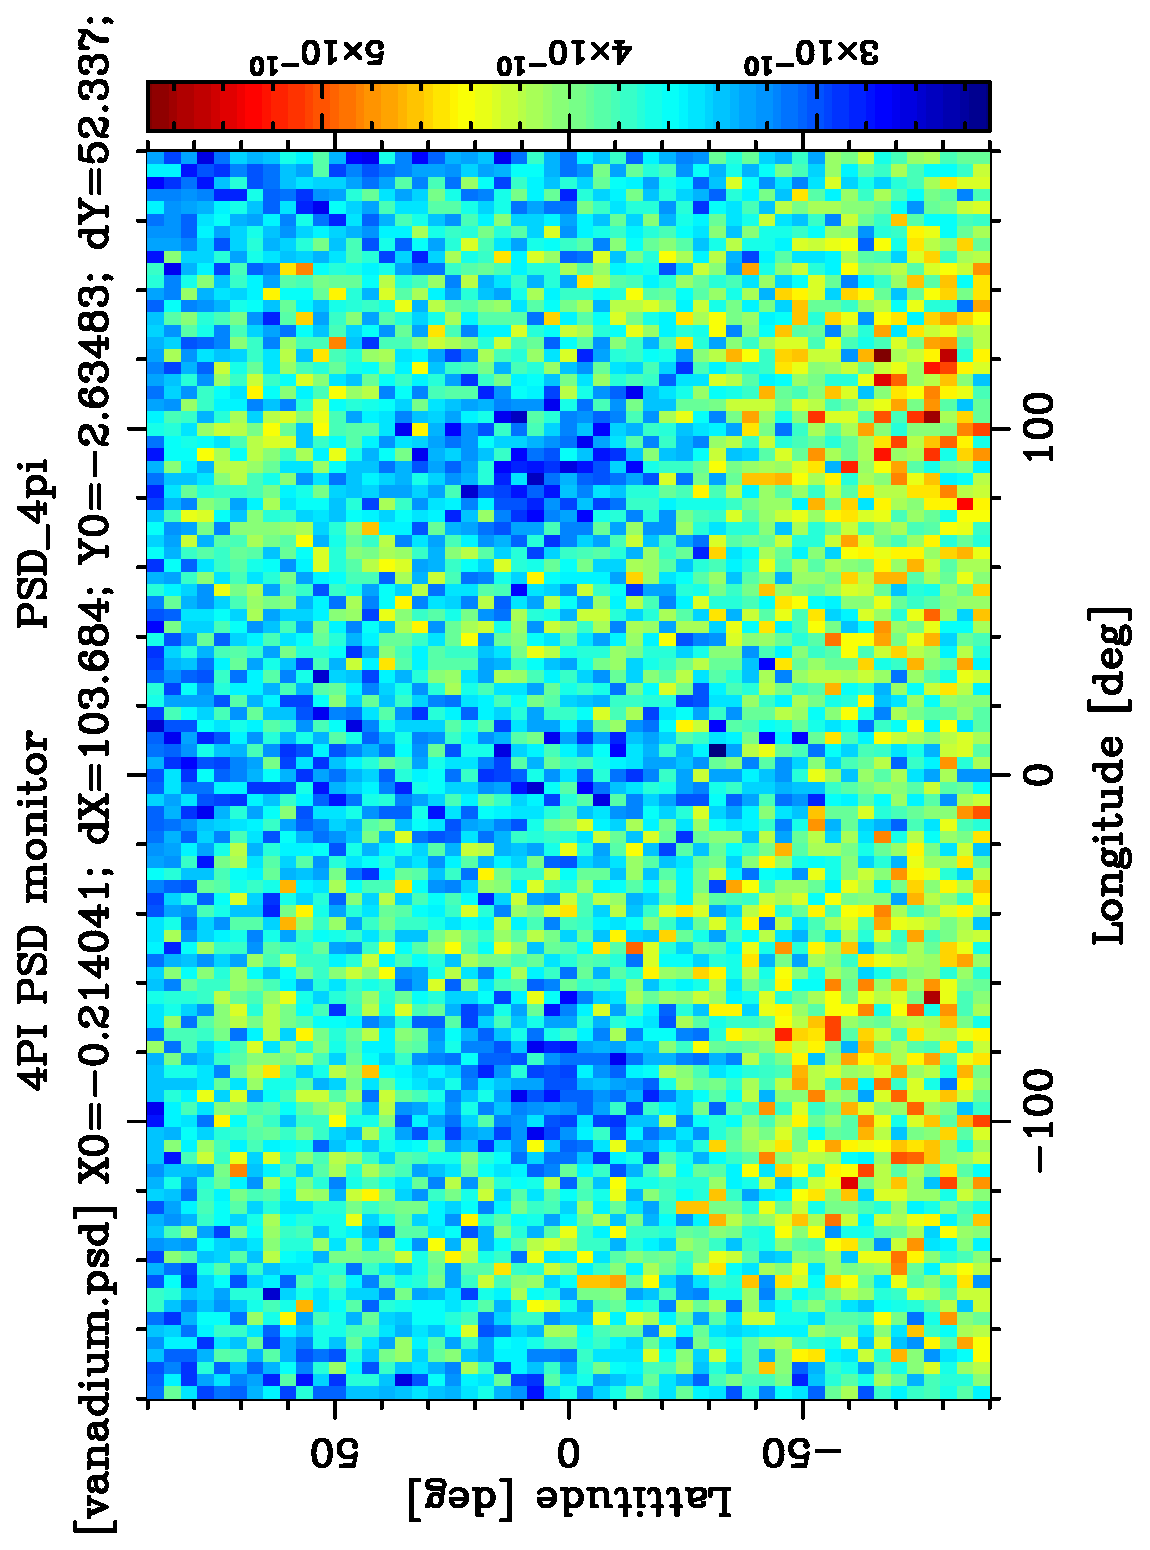
\includegraphics[angle=-90,width=1\textwidth]{figures/mcplot_PGPLOT.ps}
    \end{minipage}
    \hfill
    \begin{minipage}{.45\textwidth}
    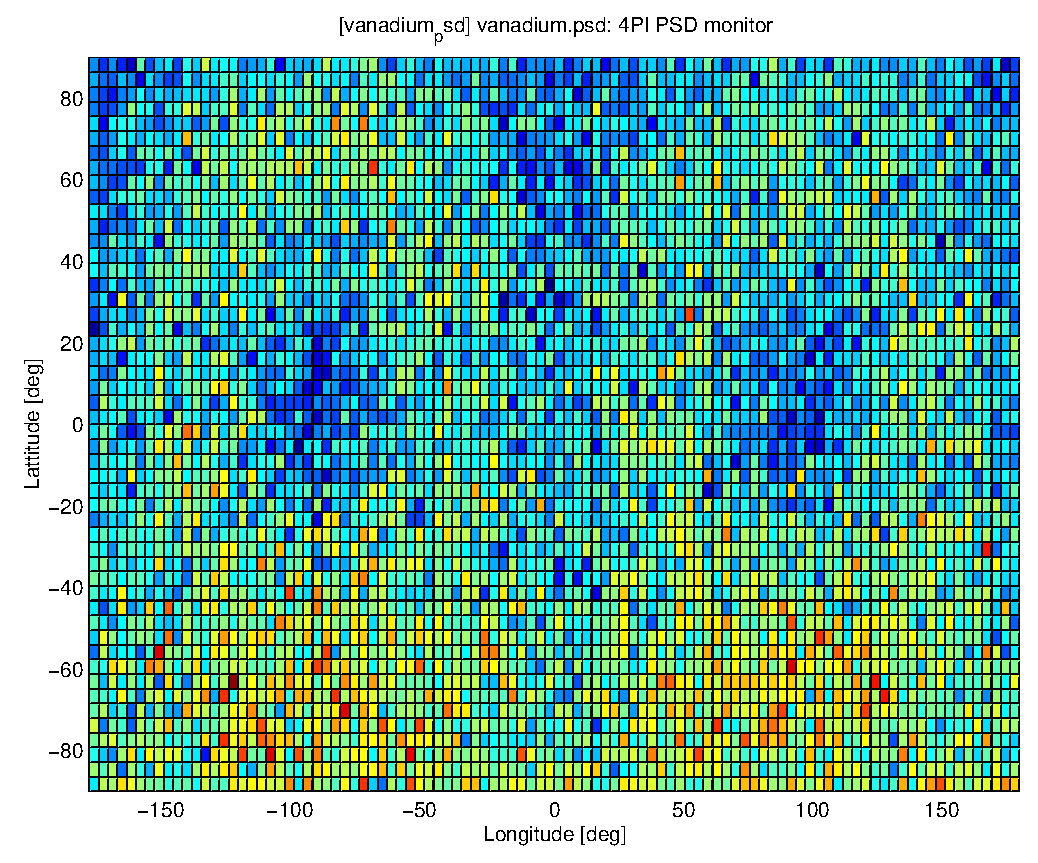
\includegraphics[width=1\textwidth]{figures/mcplot_Matlab.eps}
    \end{minipage}
\caption{Output from \texttt{mcplot} with PGPLOT and Matlab backends}
\label{fig:mcplot_figs}
\end{figure}
When using the Matlab backend, full 3D view of plots and different
display possibilities are available. Use the attached \MCS window menus to
control these. Features are quite self explanatory. For other options, execute
\verb+mcplot --help+ (\verb+mcplot.pl --help+ on windows) to get help.

\indexTOOL{PGPLOT}
\indexTOOL{Matlab}
To visualize or
debug the simulation graphically, repeat the steps but check the ``Trace''
option instead of the ``Simulate'' option.  A window will pop up showing a
sketch of the instrument.  Depending on your chosen plotting backend, the
presented graphics will resemble one of those shown in figures
\ref{fig:mcdisp_PGPLOT}-\ref{fig:mcdisp_Matlab}.
\begin{figure}[htb!]
  \begin{center}
    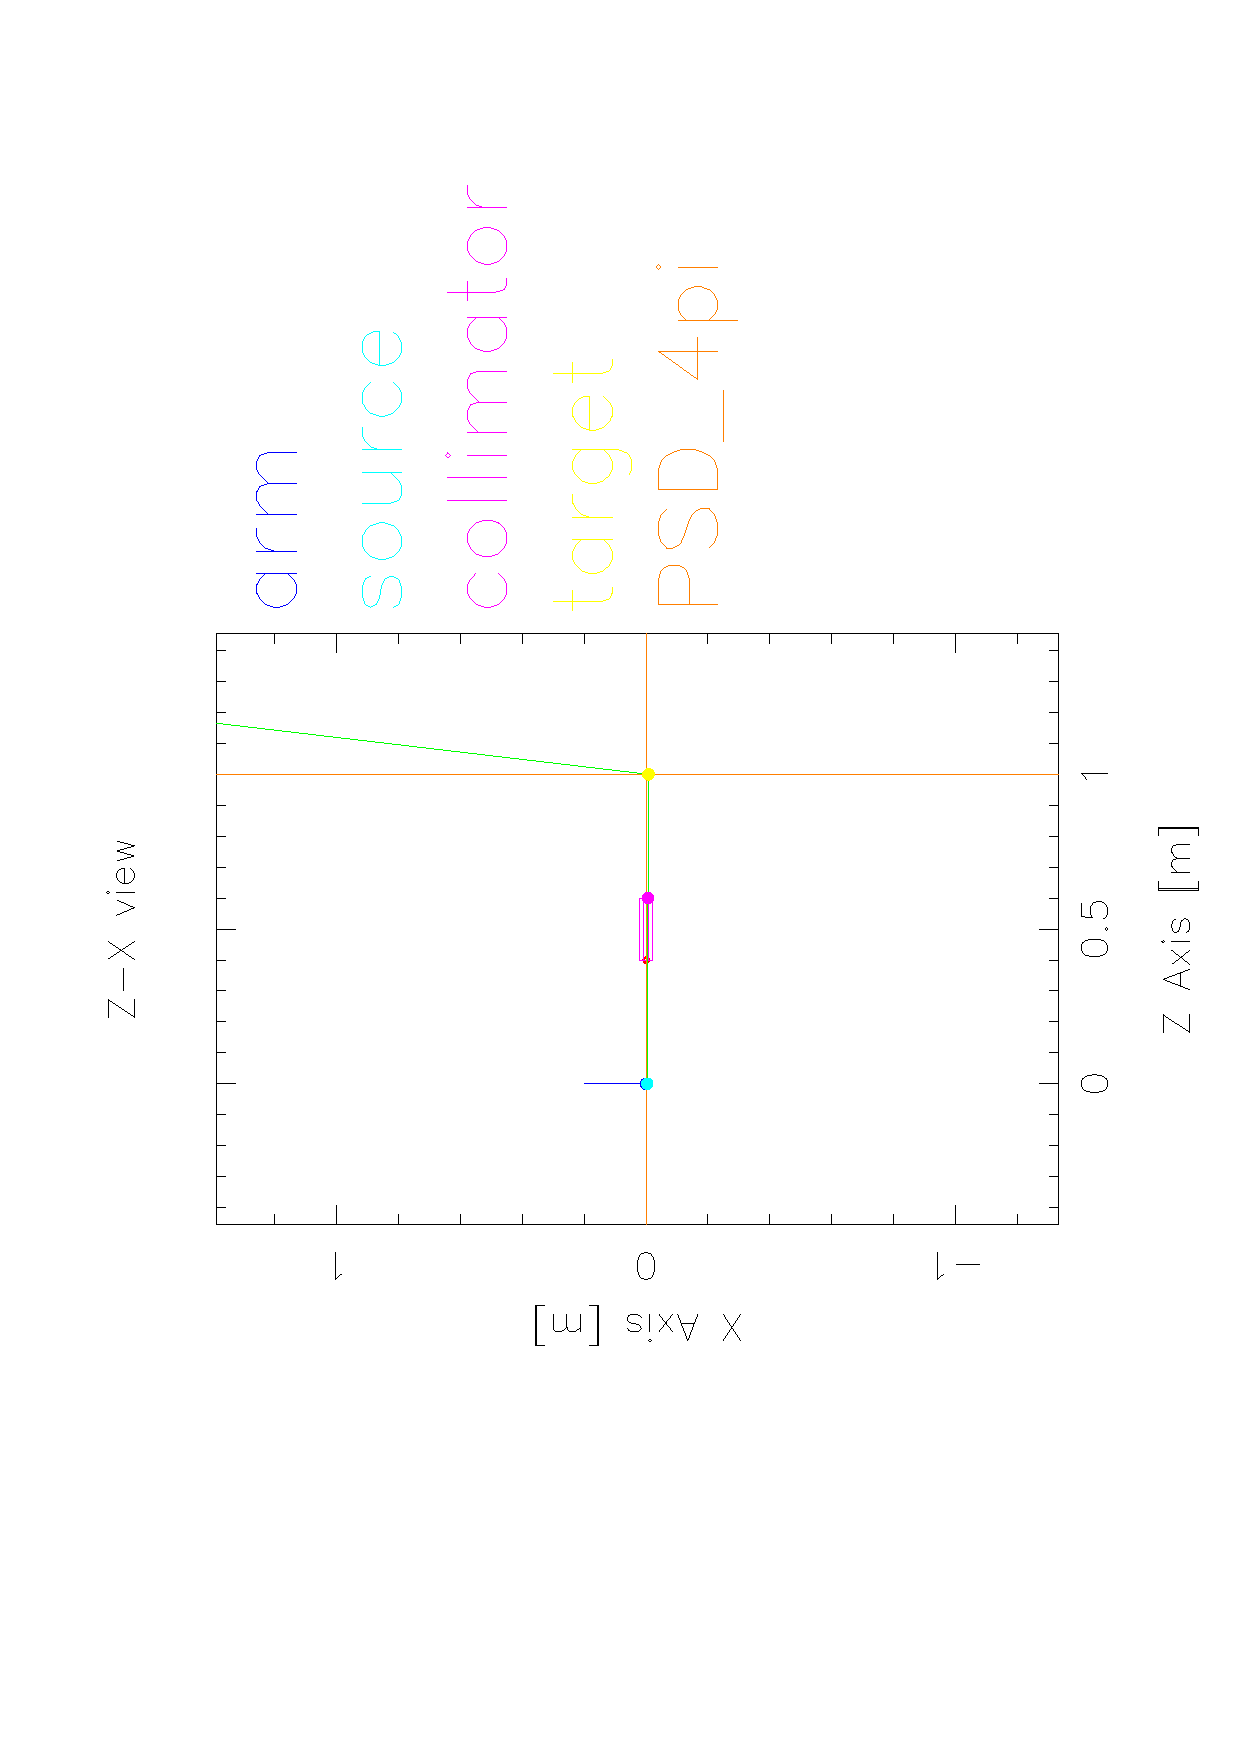
\includegraphics[width=0.48\textwidth]{figures/mcdisplay_PGPLOT}
    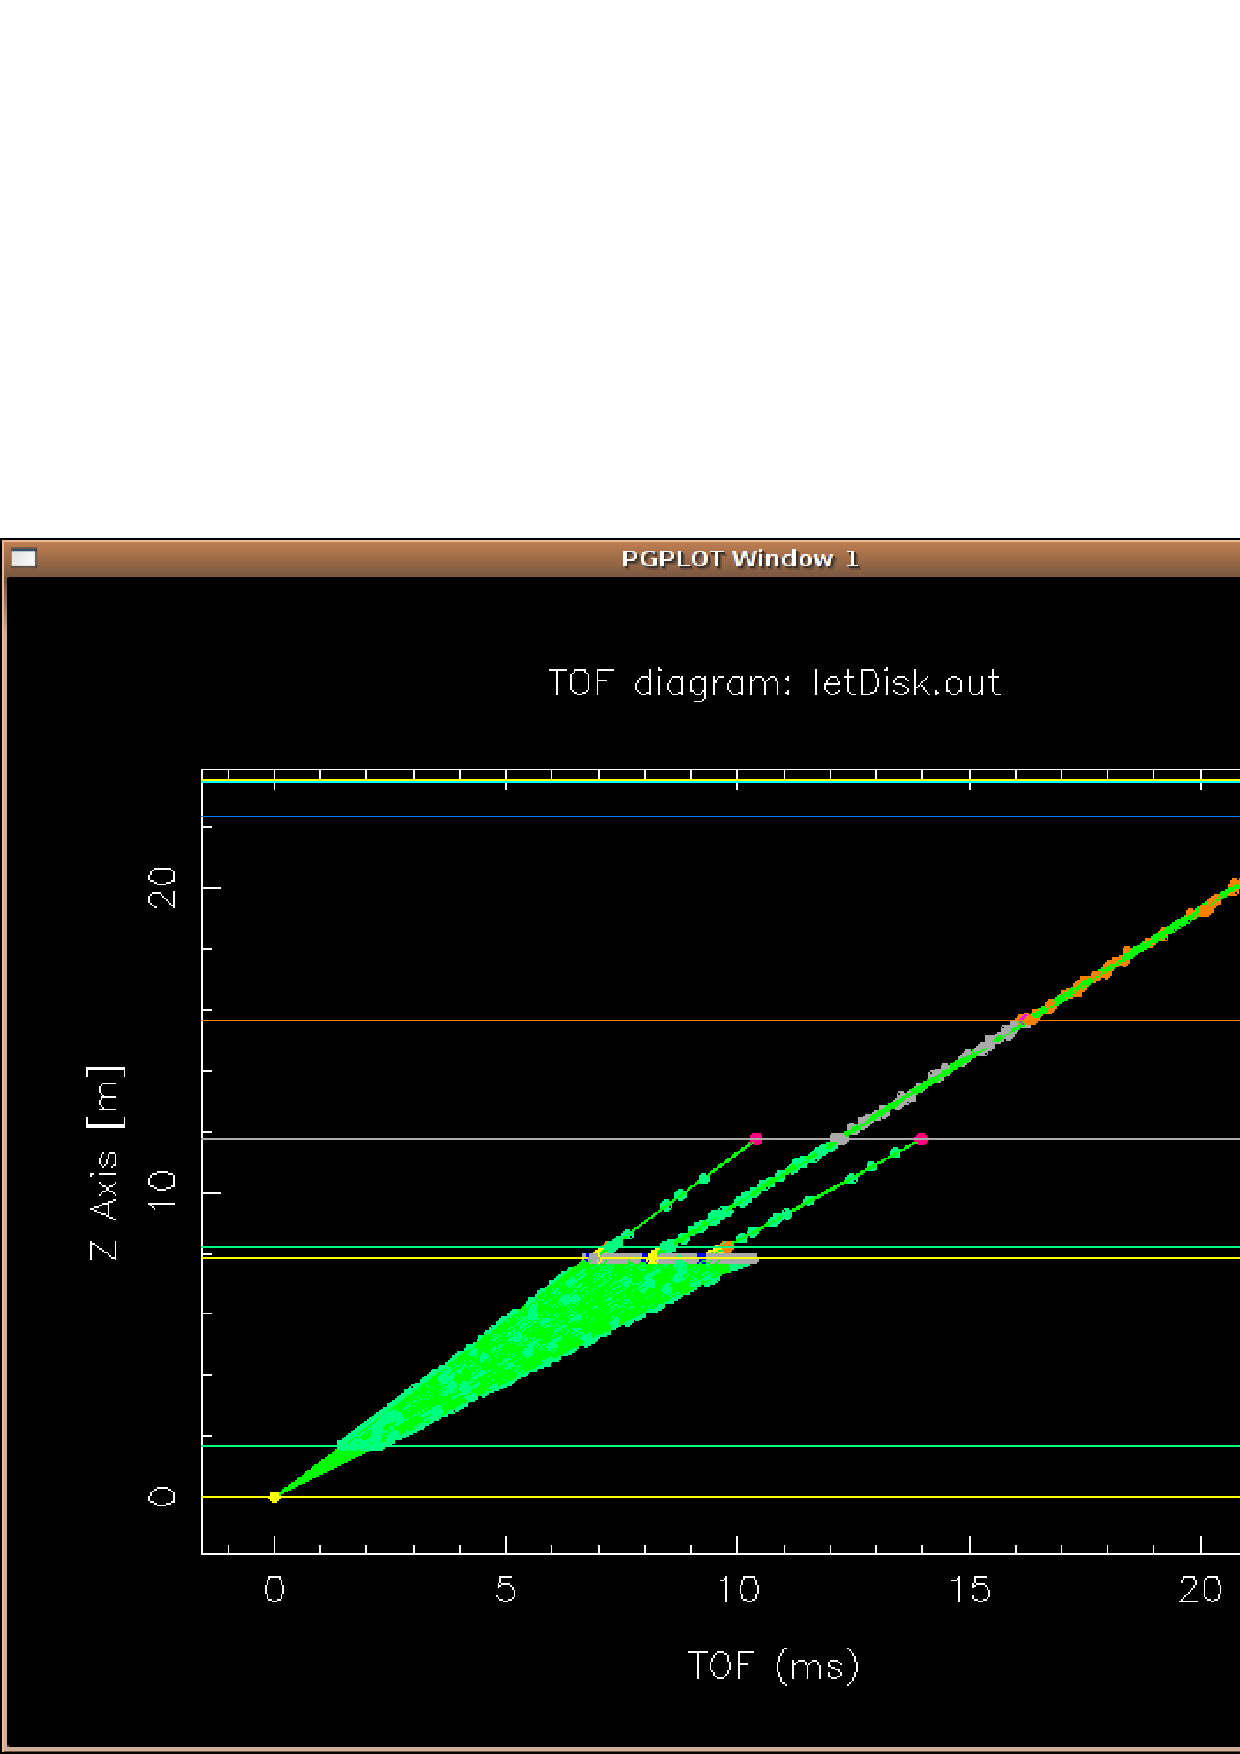
\includegraphics[width=0.48\textwidth]{figures/mcdisplay_TOF}
  \end{center}
  \caption{Left: Output from \texttt{mcdisplay} with PGPLOT backend.  The left
    mouse button starts a new neutron ray, the middle button zooms, and the
    right button resets the zoom. The Q key quits the program. Right: The new
    PGPLOT time-of-flight option. See section \ref{s:mcdisplay} for details.}
\label{fig:mcdisp_PGPLOT}
\end{figure}
\begin{figure}[htb!]
  \begin{center}
    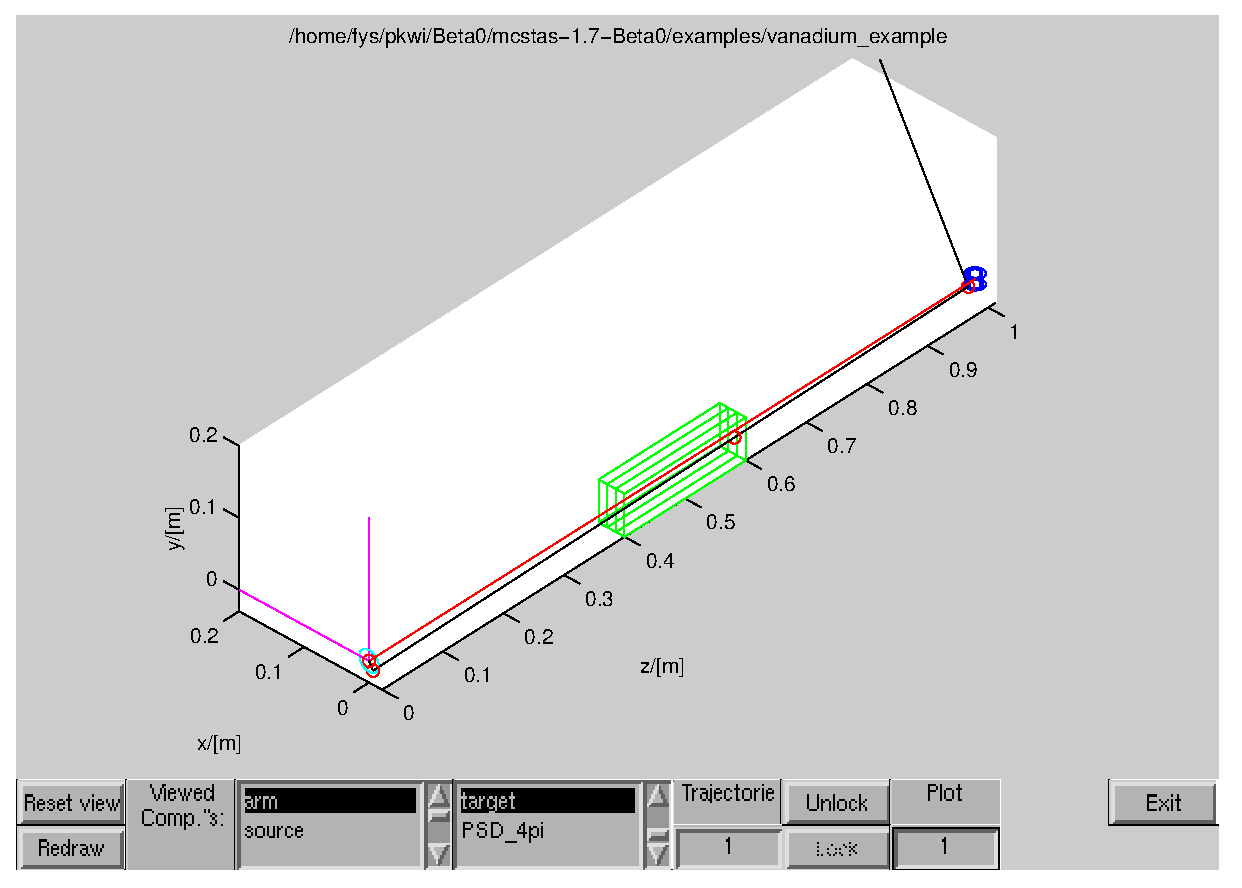
\includegraphics[width=0.55\textwidth]{figures/mcdisplay_Matlab}
  \end{center}
  \caption{Output from \texttt{mcdisplay} with Matlab backend. Display can be
    adjusted using the window buttons.}
\label{fig:mcdisp_Matlab}
\end{figure}

For a slightly longer gentle introduction to McStas, see the McStas tutorial
(available from~\cite{mcstas_webpage}), and as of version \version\ built into
the \verb+mcgui+ help menu. For more technical details, read on from
section~\ref{s:running}

\indexTOOL{mcgui|)}
\index{McStas!running through the GUI|)}


%%%%%%%%%%%%%%%%%%%%%%%%%%%%%%%%%%%%%%%%%%%%%%%%%%%%%%%%%%%%%%%%%%%%%%%%%%%%%%%%
\section{Running the instrument compiler}
\label{s:running}

\index{Compilation!instrument definition|see{mcstas (compiler)}}
\index{mcstas (compiler)|(textbf}
This section describes how to run the McStas compiler manually. Often,
it will be more convenient to use the front-end program \verb+mcgui+
(section~\ref{s:mcgui}) or \verb+mcrun+ (section~\ref{s:mcrun}). These
front-ends will compile and run the simulations automatically.

The compiler for the \MCS{} instrument definition
is invoked by typing a command of the form
\begin{bash}
    mcstas name.instr
\end{bash}
This will read the instrument definition \verb+name.instr+ which is
written in the \MCS meta-language. The compiler will translate the
instrument definition into a Monte Carlo simulation program provided in
ISO-C. The output is by default written to a file in the current
directory with the same name as the instrument file, but with extension
\verb+.c+ rather than \verb+.instr+. This can be overridden using the
\verb+-o+ option as follows:
\begin{bash}
    mcstas -o code.c name.instr
\end{bash}
which gives the output in the file \verb+code.c+.
A single dash `\verb+-+' may be used for both input and output filename
to represent standard input and standard output, respectively.


%-------------------------------------------------------------------------------
\subsection{Code generation options}
\index{Code generation!options}

By default, the output files from the \MCS compiler are in ISO-C with
some extensions (currently the only extension is the creation of new
directories, which is not possible in pure ISO-C). The use of
extensions may be disabled with the \verb+-p+ or \verb+--portable+
option. With this option, the output is strictly ISO-C compliant, at
the cost of some slight reduction in capabilities.

The \verb+-t+ or \verb+--trace+ option puts special ``trace'' code in
the output. This code makes it possible to get a complete trace of the
path of every neutron ray through the instrument, as well as the position
and orientation of every component. This option is mainly used with the
\verb+mcdisplay+ front-end as described in section~\ref{s:mcdisplay}.

The code generation options can also be controlled by using preprocessor
macros in the C compiler, without the need to re-run the \MCS
compiler. If the preprocessor macro \verb+MC_PORTABLE+ is defined, the
same result is obtained as with the \verb+--portable+ option of the
\MCS compiler. The effect of the \verb+--trace+ option may be obtained
by defining the \verb+MC_TRACE_ENABLED+ macro. Most Unix-like C
compilers allow preprocessor macros to be defined using the \verb+-D+
option, e.g.
\begin{bash}
    cc -DMC_TRACE_ENABLED -DMC_PORTABLE ...
\end{bash}
Finally, the \verb+--verbose+ option will list the components and libraries being
included in the instrument.

%-------------------------------------------------------------------------------
\subsection{Specifying the location of files}
\label{s:files}

The \MCS compiler needs to be able to find various files during compilation,
some explicitly requested by the user (such as component definitions and files
referenced by \verb+%include+), \indexKW{\%include}
and some used internally to generate the simulation executable. \MCS looks for
these files in three places: first in the current directory, then in a list of
directories given by the user, and finally in a special \MCS
directory. Usually, the user will not need to worry about this as \MCS will
automatically find the required files. But if users build their own component
library in a separate directory or if \MCS is installed in an unusual way, it
will be necessary to tell the compiler where to look for the files.

\index{Library!Components} The location of the special \MCS directory is set
when \MCS is compiled. It defaults to \verb+/usr/local/lib/mcstas+ on Unix-like
systems and \verb+C:\mcstas\lib+ on Windows systems, but it can be changed to
something else, see section~\ref{s:install} for details. The location can be
overridden by setting the environment variable \verb+MCSTAS+:
\indexEV{MCSTAS}
\begin{bash}
    setenv MCSTAS /home/joe/mcstas
\end{bash}
for csh/tcsh users, or
\begin{bash}
    export MCSTAS=/home/joe/mcstas
\end{bash}
for bash/Bourne shell users.  For Windows Users, you should define the
\verb+MCSTAS+ from the menu 'Start/Settings/Control
Panel/System/Advanced/Environment Variables' by creating \verb+MCSTAS+ with the
value \verb+C:\mcstas\lib+

To make \MCS search additional directories for component definitions
and include files, use the \verb+-I+ switch for the \MCS compiler:
\begin{lstlisting}
    mcstas -I/home/joe/components -I/home/joe/neutron/include name.instr
\end{lstlisting}
Multiple \verb+-I+ options can be given, as shown.

\index{mcstas (compiler)|)}

%-------------------------------------------------------------------------------
\subsection{Embedding the generated simulations in other programs}

By default, \MCS will generate a stand-alone C program, which is what is needed
in most cases. However, for advanced usage, such as embedding the generated
simulation in another program or even including two or more simulations in the
same program, a stand-alone program is not appropriate. For such usage, the
\MCS compiler provides the following options:
\begin{itemize}
\item \verb+--no-main+ This option makes \MCS omit the \verb+main()+ function
  in the generated simulation program. The user must then arrange for the
  function \verb+mcstas_main()+ to be called in some way.
\item \verb+--no-runtime+ Normally, the
  generated simulation program contains all the run-time C code necessary for
  declaring functions, variables, etc. used during the simulation.  This
  option makes \MCS omit the run-time code from the generated
  simulation program, and the user must then explicitly link with the file
  \verb+mcstas-r.c+ as well as other shared libraries from the \MCS{} distribution.
  \index{Library!run-time}
\end{itemize}
Users that need these options are encouraged to contact the authors for further
help.


%-------------------------------------------------------------------------------
\subsection{Running the C compiler}
\label{s:compile}

After the source code for the simulation program has been generated with the
\MCS compiler, it must be compiled with the C compiler to produce an
executable. The generated C code obeys the ISO-C standard, so it should be easy
to compile it using any ISO-C (or C++) compiler. \textit{E.g}.\ a typical
Unix-style command would be
\begin{lstlisting}
    cc -O -o name.out name.c -lm
\end{lstlisting}
The \MCS team recommends these compiler alternatives for the Intel (and AMD)
hardware architectures:
\begin{itemize}
\item[\textbf{A}]{\verb+gcc+ which is a very portable, open source, ISO-C compatible
    c compiler, available for most platforms. For Linux it is usually part of
    your distribution, for Windows the \MCS distribution package includes a
    version of \verb+gcc+ (in the Dev-CPP sub-package), and for Mac OS X
    \verb+gcc+ is part of the Xcode tools package available on the installation
    medium.}
\item[\textbf{B}]{\verb+icc+ or the Intel c compiler is available for Linux, Mac OS
    and Windows systems and is a commercial software product. Generally,
    simulations run with the Intel compiler are \textbf{a factor of 2 faster} than
    the identical simulation run using \verb+gcc+. To use \verb+icc+ with \MCS
    on Linux or Mac OS X, set the environment variables
    \begin{itemize}
      \item{\verb+MCSTAS_CC=icc+}
      \item{\verb+MCSTAS_CFLAGS="-g -O2 -wd177,266,1011,181"+}
    \end{itemize}
    To use \verb+icc+ with MPI on Unix system (see Section \ref{s:run-mpi})
 installations, it seems that \emph{editing}
    the mpicc shell script and setting the CC variable to "\verb+icc+" is the
    only requirement!}
  On Windows, the Intel c compiler is 'icl', not 'icc' and has a dependency for
  Microsoft Visual C++. If you have both these softwares available, running
  McStas with the Intel compiler should be possible (currently untested by the
  McStas developer team).

\end{itemize}


The \verb+-O+ option typically enables the optimization phase of the compiler,
which can make quite a difference in speed of \MCS generated simulations. The
\verb+-o name.out+ sets the name of the generated executable. The \verb+-lm+
options is needed on many systems to link in the math runtime library (like the
$\cos()$ and $\sin()$ functions). \index{Optimization!compiler option}

Monte Carlo simulations are computationally intensive, and it is often desirable
to have them run as fast as possible. Some success can be obtained by adjusting
the compiler optimization options. Here are some example platform and compiler
combinations that have been found to perform well (up-to-date information will
be available on the \MCS WWW home page~\cite{mcstas_webpage}):
\begin{itemize}
\item Intel x86 (``PC'') with Linux and GCC, using options \verb+gcc -O3+.
\item Intel x86 with Linux and EGCS (GCC derivate) using
  options \verb+egcc -O6+.
\item Intel x86 with Linux and PGCC (pentium-optimized GCC derivate), using
  options \verb+gcc -O6 -mstack-align-double+.
\item HPPA machines running HPUX with the optional ISO-C compiler,
  using the options
  \verb|-Aa +Oall -Wl,-a,archive| (the \verb+-Aa+ option is necessary to
  enable the ISO-C standard).
\item SGI machines running Irix with the options
  \verb|-Ofast -o32 -w|
\end{itemize}
Optimization flags will typically result in a speed improvement by a factor
about 3, but the compilation of the instrument may be 5 times slower.

A warning is in place here: it is tempting to spend far more time fiddling with
compiler options and benchmarking than is actually saved in computation
times. Even worse, compiler optimizations are notoriously buggy; the options
given above for PGCC on Linux and the ISO-C compiler for HPUX have been known to
generate \emph{incorrect code} in some compiler versions. \MCS actually puts an
effort into making the task of the C compiler easier, by in-lining code and
using variables in an efficient way. As a result, \MCS simulations generally
run quite fast, often fast enough that further optimizations are not
worthwhile. Also, optimizations are highly time and memory consuming during
compilation, and thus may fail when dealing with large instrument descriptions
(e.g. more that 100 elements). The compilation process is simplified when using
components of the library making use of shared libraries (see \verb+SHARE+
keyword in chapter~\ref{c:kernel}). Refer to section \ref{s:optim} for other
optimization methods.\index{Optimization}

%%%%%%%%%%%%%%%%%%%%%%%%%%%%%%%%%%%%%%%%%%%%%%%%%%%%%%%%%%%%%%%%%%%%%%%%%%%%%%%%
\section{Running the simulations}
\label{s:run-sim}
\index{Parameters!instruments}

Once the simulation program has been generated by the \MCS compiler
and an executable has been obtained with the C compiler, the simulation
can be run in various ways.

\subsubsection{Simple McStas options}
In this section, the most common simulation parameters are
discussed. For a full list, please consult tables
\ref{f:simoptions,f:simoptions2}

The simplest way is to run it directly from the
command line or shell:
\begin{lstlisting}
    ./name.out
\end{lstlisting}
Note the leading ``.'', which is needed if the current directory is not in the
path searched by the shell. When used in this way, the simulation will prompt
for the values of any instrument parameters such as angular settings, and then
run the simulation. Default instrument parameter values (see
section~\ref{s:instrdefs}), if any, will be indicated and entered when hitting
the \verb+Return+ key.\index{Parameters!optional, default value} This way of
running \MCS will only give data for one instrument setting which is normally
sufficient for {\em e.g.}, time-of-flight, SANS or powder instruments, but not
for {\em e.g.} continuous-beam reflectometers or triple-axis spectrometers where
a scan over various instrument settings is required.  Often the simulation will
be run using one of several available front-ends, as described in the next
section. These front-ends help manage output from the potentially many detectors
in the instruments, as well as running the simulation for each data point in a
scan.

The generated simulations accept a number of options and arguments. The
full list can be obtained using the \verb+--help+ option:
\begin{lstlisting}
    ./name.out --help
\end{lstlisting}
The values of instrument parameters may be specified as arguments using
the syntax \textit{name}\verb+=+\textit{val}. For example
\begin{lstlisting}
    ./Samples_vanadium.out ROT=90
\end{lstlisting}
\index{Parameters!instruments}
The number of neutron histories to simulate may be set using the
\verb+--ncount+ or \verb+-n+ option, for example
\verb+--ncount=2e5+. The initial seed for the random number generator is
by default chosen based on the current time so that it is different for
each run. However, for debugging purposes it is sometimes convenient to
use the same seed for several runs, so that the same sequence of random
numbers is used each time. To achieve this, the random seed may be set
using the \verb+--seed+ or \verb+-s+ option.

By default, \MCS simulations write their results into several data files in the
current directory, overwriting any previous files stored there. The
\verb+--dir=+\textit{dir} or \verb+-d+\textit{dir} option causes the files to be
placed instead in a newly created directory \textit{dir} (to prevent overwriting
previous results an error message is given if the directory already exists).
Alternatively, all output may be written to a single file \textit{file} using
the \verb+--file=+\textit{file} or \verb+-f+\textit{file} option (which should
probably be avoided when saving in binary format, see below). If the \verb+file+
is given as \verb+NULL+, the file name is automatically built from the
instrument name and a time stamp. The default file name is \verb+mcstas+
followed by appropriate extension.

The complete list of options
and arguments accepted by \MCS simulations appears in
Tables \ref{f:simoptions} and \ref{f:simoptions2}.

%-------------------------------------------------------------------------------
\subsection{Choosing an output data file format}

Data files contain header lines with information about the simulation from which
they originate. In case the data must be analyzed with programs that cannot read
files with such headers, they may be turned off using the \verb+--data-only+ or
\verb+-a+ option.  \index{Data formats}\index{Formats|see{Data formats}}

The format of the output files from \MCS simulations is described in more
detail in section~\ref{s:analyze}. It may be chosen either with
\verb+--format=FORMAT+ for each simulation or globally by setting the
MCSTAS\_FORMAT environment variable.
\indexEV{MCSTAS\_FORMAT}
The available format list is obtained using the \verb+name.out --help+ option.
\indexTOOL{PGPLOT}
\indexTOOL{Matlab}
\index{Data formats}
\MCS can presently generate the \MCS /PGPLOT and the NeXus format. 

It is also possible to create and read \textit{Vitess}, \textit{MCNP/PTRAC} and
\textit{Tripoli4/batch} neutron event files using components
\begin{itemize}
\item \verb+Vitess_input+ and \verb+Vitess_output+
\item \verb+Virtual_tripoli4_input+ and \verb+Virtual_tripoli4_output+
\item \verb+Virtual_mcnp_input+ and \verb+Virtual_mcnp_output+
\end{itemize}\index{Vitess} \index{Tripoli} \index{MCNP}

Additionally, adding the \texttt{raw} keyword to the FORMAT will produce raw
$[N, p, p^2]$ data sets instead of $[N, p, \sigma]$ (see Section
\ref{s:staterror}). The former representation is fully additive, and thus
enables to add results from separate simulations (e.g. when using a computer
Grid - which is automated in the \verb+mcformat+ tool). Other acceptable format
modifiers are \verb+transpose+ to transpose data matrices and \verb+append+ to
concatenate data to existing files.

%-------------------------------------------------------------------------------
\subsection{Basic import and plot of results}
\label{s:run-format}
The previous example will result in a \verb+mcstas.sim+ file, that may be read
directly from Matlab (using the \textit{sim file} function)
\begin{matlab}
    matlab> s=mcstas;
    matlab> s=mcstas('plot')
\end{matlab}
\indexTOOL{Matlab}
The first line returns the simulation data as a single structure variable,
whereas the second one will additionally plot each detector separately.  This
also equivalently stands for IDL 
\begin{lstlisting}
    idl> s=mcstas()
    idl> s=mcstas(/plot)
\end{lstlisting}
\indexTOOL{IDL}
See section~\ref{s:mcplot} for another way of plotting simulation results
using the \verb+mcplot+ front-end.
\indexTOOL{mcplot}

When choosing the HTML format, the simulation results are saved as a web page,
whereas the monitor data files are saved as VRML files, displayed within the web
page.
\indexTOOL{VRML/OpenGL}\index{OpenGL}

\begin{table}
  \begin{center}
    {\let\my=\\
    \begin{tabular}{|p{0.24\textwidth}|p{0.7\textwidth}|}
      \hline
      \texttt{-s \textit{seed}} \my \texttt{--seed=\textit{seed}}
        & Set the initial seed for the random number generator. This may be
        useful for testing to make each run use the same random number
      sequence. \\
      \hline
      \texttt{-n \textit{count}} \my \texttt{--ncount=\textit{count}}
        & Set the number of neutron histories to simulate. The default
      is 1,000,000. (1e6)\\
      \hline
      \texttt{-d \textit{dir}} \my \texttt{--dir=\textit{dir}}
        & Create a new directory \textit{dir\/} and put all data files in
      that directory. \\
      \hline
      \texttt{-h} \my \texttt{--help}
        & Show a short help message with the options accepted, available formats
        and the names of the parameters of the instrument. \\
      \hline
      \texttt{-i} \my \texttt{--info}
        & Show extensive information on the simulation and the
      instrument definition it was generated from. \\
      \hline
      \texttt{-t} \my \texttt{--trace}
        & Makes the simulation output the state of every
      neutron as it passes through every component. Requires that the
      \texttt{-t} (or \texttt{--trace}) option is also given to the
      \MCS compiler when the simulation is generated. \\
      \hline
      \texttt{--no-output-files}
        & Disables the writing of data files (output to the
      terminal, such as detector intensities, will still be written). \\
      \hline
      \texttt{-g} \my \texttt{--gravitation}
        & Toggles the gravitation (approximation) handling
        for the whole neutron propagation within the instrument. May
        produce wrong results if the used components do no comply with
        this option.\\
      \hline
      \texttt{--format=\textit{FORMAT}}
        & Sets the file format for result simulation and data files. \\
      \hline
      \texttt{-N \textit{STEPS}}
        & Divide simulation into STEPS, varying parameters within given ranges 'min,max'. \\
      \hline
      \texttt{\textit{param}{\texttt =}\textit{value} \my \textit{min,max}}
        & Set the value of an instrument parameter, rather than having
        to prompt for each one. Scans ranges are specified as 'min,max'.\\
      \hline
    \end{tabular}
    \caption{Options accepted by \MCS simulations. For options
      specific to MPI and parallel computing, see section \ref{s:run-mpi}.}
    \label{f:simoptions}
    }
  \end{center}
\end{table}

\begin{table}
  \begin{center}
    {\let\my=\\
    \begin{tabular}{|p{0.35\textwidth}|p{0.6\textwidth}|}
      \hline
      \texttt{-f \textit{file}} \my \texttt{--file=\textit{file}}
        & Write all data into a single file \textit{file}. Avoid when using binary formats. \\
      \hline
      \texttt{--format\_data=\textit{FORMAT}}
        & Sets the file format for result data files from monitors. This enables to have simulation files in one format (e.g. HTML), and monitor files in an other format (e.g. VRML).\\
      \hline
      \texttt{--mpi=\textit{NB\_CPU}}
        & Distributes the simulation over NB\_CPU node (requires MPI
        to be installed). Speedup has been demonstrated to be linear
        in number of nodes when the simulation task is \verb+--ncount+
        is sufficiently large.\\
      \hline
      \texttt{--multi=\textit{NB\_CPU}} \my \texttt{--grid=\textit{NB\_CPU}}
        & Distributes the simulation over NB\_CPU node (requires SSH to be installed). Speedup has been demonstrated to be linear
        in number of nodes when the simulation task is \verb+--ncount+
        is sufficiently large.\\
      \hline
      \texttt{--machines=\textit{MACHINES}}
        & Specify a list of distant machines/nodes to be used for MPI and grid clustering. Default is to use local SMP cluster.\\
      \hline
      \texttt{--optim}
        & Run in optimization mode to find best parameters in order to maximize all monitor integral values. Parameters to be varied are given just like scans (min,max).\\
      \hline
      \texttt{--optim=\textit{COMP}}
        & Same as \verb+--optim+ but for specified monitors. This option may be used more than once.\\
      \hline
      \texttt{--optim-prec=\textit{ACCURACY}}
        & Sets accuracy criteria to end parameter optimization (default is 10$^{-3}$).\\
      \hline
      \texttt{--test}
        & Run \MCS self test.\\
      \hline
      \texttt{-c} \my \texttt{--force-compile}
        & Force to recompile the instrument.\\
      \hline
    \end{tabular}
    \caption{Additional options accepted by \MCS simulations.}
    \label{f:simoptions2}
    }
  \end{center}
\end{table}

%-------------------------------------------------------------------------------
\subsection{Interacting with a running simulation}
\index{Signal handler|textbf}

Once the simulation has started, it is possible, under Unix, Linux and Mac OS X systems, to interact with the on-going simulation. This feature is not available when using MPI parallelization.

\MCS attaches a signal handler to the simulation process. In order to send a signal to the process, the process-id \textit{pid} must be known. Users may look at their running processes with the Unix 'ps' command, or alternatively process managers like 'top' and 'gtop'.
If a \textit{file.out} simulation obtained from \MCS is running, the process status command should output a line resembling

\begin{bash}
<user> 13277 7140 99 23:52 pts/2   00:00:13   file.out
\end{bash}

where \verb+user+ is your Unix login. The \textit{pid} is there '13277'.

Once known, it is possible to send one of the signals listed in Table~\ref{t:signals} using the 'kill' unix command (or the functionalities of your process manager), e.g.
\begin{bash}
    kill -USR2 13277
\end{bash}

This will result in a message showing status (here 33 \% achieved), as well as the position in the instrument of the current neutron.
\begin{lstlisting}
# McStas: [pid 13277] Signal 12 detected SIGUSR2 (Save simulation)
# Simulation: file (file.instr)
# Breakpoint: MyDetector (Trace) 33.37 % (  333654.0/ 1000000.0)
# Date      : Wed May  7 00:00:52 2003
# McStas: Saving data and resume simulation (continue)
\end{lstlisting}
followed by the list of detector outputs (integrated counts and files). Finally, sending a \verb+kill 13277+ (which is equivalent to \verb+kill -TERM 13277+) will end the simulation before the initial 'ncount' preset.

A typical usage example would be, for instance, to save data during a
simulation, plot or analyze it, and decide to interrupt the simulation earlier
if the desired statistics has been achieved. This may be done automatically
using the \verb+Progress_bar+ component.

Whenever simulation data is generated before end (or the simulation is
interrupted), the 'ratio' field of the monitored data will provide the level of
achievement of the computation (for instance '3.33e+05/1e+06'). Intensities are
then usually to be scaled accordingly by the user.

Additionally, any system error will result in similar messages, giving
indication about the occurrence of the error (component and section). Whenever
possible, the simulation will {\em try} to save the data before ending. Most
errors appear when using a newly written component, in the \texttt{INITIALIZE},
\texttt{TRACE} or \texttt{FINALLY} sections. Memory errors usually show up when
C pointers have not been allocated/unallocated before usage, whereas
mathematical errors are found when, for instance, dividing by zero.

\begin{table}
  \begin{center}
    {\let\my=\\
    \begin{tabular}{|p{0.24\textwidth}|p{0.7\textwidth}|}
      \hline
      \texttt{USR1} & Request information (status)  \\
      \texttt{USR2, HUP} & Request information and performs an intermediate
      saving of all monitors (status and save). This triggers the execution of
      all \texttt{SAVE} sections (see chapter~\ref{c:kernel}).  \\
      \texttt{INT, TERM} & Save and exit before end (status)  \\
      \hline
    \end{tabular}
    \caption{Signals supported by \MCS simulations.}
    \label{t:signals}
    }
  \end{center}
\end{table}

%-------------------------------------------------------------------------------
\subsection{Optimizing simulation speed}
\index{Optimization|textbf}
\label{s:optim}
There are various ways to speed up simulations
\begin{itemize}
\item Optimize the compilation of the instrument, as explained in
  section~\ref{s:compile}.
\item Execute the simulation in parallel on a computer grid or a cluster (with
  MPI or ssh grid ) as explained in section~\ref{s:run-mpi}.
\item Divide simulation into parts using a file for saving or generating neutron
  events. In this way, a guide may be simulated only once, saving the neutron
  events at the guide exit as a file, which is being read quickly by the second
  simulation part. Use the Virtual\_input and Virtual\_output components for
  this technique.
\item Use source optimizers like the components Source\_adapt or
  Source\_Optimizer. Such component may sometimes not be very efficient, when no
  neutron importance sampling can be achieved, or may even sometimes alter the
  simulation results. Be careful and always check results with a (shorter)
  non-optimized computation.
\item Complex components usually take into account additional small effects in a
  simulation, but are much longer to execute. Thus, simple components should be
  preferred whenever possible, at least in the beginning of a simulation project.
\item The SPLIT keyword may artificially repeat events reaching specified
  positions in the instrument. This is \emph{very} efficient, but requires to
  cast random numbers in the course of the remaining propagation (e.g. at
  samples, crystals, ...). See section \ref{s:instrdefs-extend-enhance} for
  details.
\end{itemize}
A general comment about optimization is that it should be used cautiously,
checking that the results are not significantly affected.

%-------------------------------------------------------------------------------
\subsection{Optimizing instrument parameters}
\label{s:optimize}\index{Parameters!optimization}
Often, the user may wish to optimize the parameters of a simulation, i.e. the
best geometry of a given component, for example the optimal curvature of a
monochromator.

The choice of the optimization routine, of the simulation quality value to
optimize, the initial parameter guess and the simulation length all have a large
influence on the results.  The user is advised to be cautious when interpreting
the optimization results.

\subsubsection{Using iFit for optimization}

One of the authors of \MCS has developed a very flexible and general data
analysis and fitting package called iFit\ref{iFit,iFit_web} based on
Matlab. Matlab itself is not required, as a stand-alone distributable binary of
iFit exists.

iFit contains wrapper functionality for compiling and running \MCS simulations
as object functions, and allows to select many different optimizers, including
swarms and other non-gradient methods. Please see the iFit documentation for
more information.

Our experience is that iFit together with \MCS is a more robust optimization
solution than the \MCS built-in Simplex solution.

\subsubsection{Using the Simplex method}

The \MCS package comes with a Simplex optimization method to find best
instrument parameters in order to maximize all or some specified monitor
integrated values. It uses the Downhill Simplex Method in
Multidimensions~\cite{neldermead,NumRecip} which is a geometric optimization
method somewhat similar to genetic algorithms. It is not as fast as the gradient
method, but is much more robust. It is well suited for problems with up to about
10-20 parameters to optimize. Higher dimensionalities are not guarantied to
converge to a meaningful solution.

When using \verb+mcrun+ (section \ref{s:mcrun}), the optimization mode is set by
using the \verb+--optim+ option or a list of monitors to maximize with as many
\verb+--optim=COMP+ as required. The optimization accuracy criterion may be
changed with the \verb+--optim-prec=accuracy+ option.

From \verb+mcgui+ (section \ref{s:mcgui}), one should choose the 'Optimization'
execution mode (instead of the Simulation or Trace mode). Then specify the
instrument parameters to optimize by indicating their variation range
\verb+param=min,max+ (e.g. Lambda=1,4) just like parameter scans. Optionally,
the starting guess value might be given with the syntax
\verb+param=min,guess,max+. The optimization accuracy criterion is controlled
using the 'Precision' entry box in the configuration options (See Figure
\ref{fig:mcgui-choose}). Finally, run the simulation. The optimum set of
parameters is then printed at the end of the simulation process. You may ask to
maximize only given monitors (instead of all) by selecting their component names
in the lower lists in the Run Dialog (up to 3).

If you would like to maximize the flux at a given monitor, with some
divergence constrains, you should for instance simply add a divergence
collimator before the monitor. Alternatively, write a new component
that produce the required 'figure-of-merit'.

The optimization search interval constrains the evolution of
parameters. It should be chosen carefully. In particular it is safer
for it to indeed contain a high signal domain, and be preferably
symmetric with respect to that maximum.

\subsubsection{Using custom optimization routines}
The user should write a function script or a program that
\begin{itemize}
\item inputs the simulation parameters, which are usually numerical values such
  as $TT$ in the \verb+prisma2+ instrument from the \verb+examples+ directory of
  the package.
\item builds a command line from these parameters.
\item executes that command, and waits until the end of the computation.
\item reads the relevant data from the monitors.
\item outputs a simulation quality measurement from this data, usually the
  integrated counts or some peak width.
\end{itemize}

For instance, for the \verb+prisma2+ instrument we could write a function for
Matlab (see section~\ref{s:analyze} for details about the Matlab data format) in
order to study the effects of the $TT$ parameter:
\begin{lstlisting}
  function y = instr_value(p)
    TT = p(1);     % p may be a vector/matrix containing many parameters
    syscmd = [ 'mcrun prisma2.instr -n1e5 TT=' num2str(TT) ...
               ' PHA=22 PHA1=-3 PHA2=-2 PHA3=-1 PHA4=0 PHA5=1' ...
               ' PHA6=2 PHA7=3 TTA=44 --format="Matlab binary"' ];
    system(syscmd); path(path) % execute simulation, and rehash files
    s = mcstas;     % get the simulation data, and the monitor data
    s = s.prisma2.m_mcstas.detector.prisma2_tof.signal;
    eval(s);        % we could also use the 'statistics' field
    y = -Mean;      % 'value' of the simulation
\end{lstlisting}

Then a numerical optimization should be available, such as those provided with Matlab, IDL, and Perl-PDL high level languages. In this example, we may wish to maximize the \verb+instr_value+ function value. The \verb+fminsearch+ function of Matlab is a minimization method (that's why we have a minus sign for $y$ value), and:
\begin{lstlisting}
    matlab> TT = fminsearch('instr_value', -25)
\end{lstlisting}
will determine the best value of TT, starting from -25 estimate, in order to
minimize function \verb+instr_value+, and thus maximize the mean detector
counts.

%%%%%%%%%%%%%%%%%%%%%%%%%%%%%%%%%%%%%%%%%%%%%%%%%%%%%%%%%%%%%%%%%%%%%%%%%%%%%%%%
\section{Using simulation front-ends}
\label{s:frontends}

\MCS includes a number of front-end programs that extend the
functionality of the simulations. A front-end program is an interface
between the user and the simulations, running the simulations and
presenting the output in various ways to the user.

The list of available \MCS front-end programs may be obtained from the
\verb+mcdoc --tools+ command:
\begin{lstlisting}
    McStas Tools
       mcstas        Main instrument compiler
       mcrun         Instrument build and execution utility
       mcgui         Graphical User Interface instrument builder
       mcdoc         Component library documentation generator/viewer
       mcplot        Simulation result viewer
       mcdisplay     Instrument geometry viewer
       mcresplot     Instrument resolution function viewer
       mcstas2vitess McStas to Vitess component translation utility
       mcformat      Conversion tool for text files and MPI/grids
       mcformatgui   GUI for mcformat
       mcdaemon      Instrument results on-line plotting
    When used with the -h flag, all tools display a specific help.
    SEE ALSO: mcstas, mcdoc, mcplot, mcrun, mcgui, mcresplot, mcstas2vitess
    DOC:      Please visit http://www.mcstas.org
\end{lstlisting}

%-------------------------------------------------------------------------------
\subsection{The graphical user interface (mcgui)}
\label{s:mcgui}
\indexTOOL{mcgui|textbf}

The front-end \verb+mcgui+ provides a graphical user interface that interfaces
the various parts of the McStas package. It may be started with the single
command
\begin{lstlisting}
    mcgui
\end{lstlisting}
The mcgui (mcgui.pl on Windows) program may optionally be given the name of the
instrument file to use.

\paragraph{Dependencies:}
\indexTOOL{PGPLOT} To run the \verb+mcgui+
front-end, the programs Perl and Perl/Tk must be properly installed on the
system. Additionally, to use the \MCS/PGPLOT back-end the software packages
PGPLOT, PgPerl, and PDL are required.
\index{Perl!libraries} It may be
necessary to set the \verb+PGPLOT_DIR+ and \verb+PGPLOT_DEV+ environment
variable; consult the documentation for PGPLOT on the local system in case of
difficulty.
\indexEV{PGPLOT\_DIR}
\indexEV{PGPLOT\_DEV}

\subsubsection{The menus}

When the front-end is started the main window is opened (see figure
\ref{fig:mcgui}). This window displays the output from compiling and running
simulations, and contains a few menus and buttons for easy navigation. The main
purpose of the front-end is to edit and compile instrument definitions, run the
simulations, and visualize the results.

The \textbf{File} menu has the following features:
\begin{description}
\item[File/Open instrument] selects the name of an instrument file to be used.
\item[File/Edit current] opens a simple editor window with McStas syntax
  highlighting for editing the
  current instrument definition. This function is also available from
  the \textbf{Edit} button to the right of the name of the instrument definition in
  the main window.
\item[File/Spawn editor] This starts the editor defined in the environment
  variable \verb+VISUAL+ or \verb+EDITOR+ on the current instrument
  file. It is also possible to start an external editor manually; in any
  case \verb+mcgui+ will recompile instrument definitions as necessary based on
  the modification dates of the files on the disk.
  \indexEV{EDITOR}
\item[File/Compile instrument] forces a recompile of the instrument definition,
  regardless of file dates. This is for example useful to pick up changes in
  component definitions, which the front-end will not notice automatically. This
  might also be required when choosing MPI \index{MPI|textbf} and NeXus options.
  \indexTOOL{NeXus}
\item[File/Save log file] saves the text in the window showing output of
  compilations and simulations into a file.
\item[File/Clear output] erases all text in the window showing output of
  compilations and simulations.
  \item[File/Preferences] Opens the choose backend dialog shown in
  figure~\ref{fig:mcgui-choose}. Several settings can be chosen here:
\begin{itemize}
  \item Selection of  the desired (PGPLOT|Matlab|HTML/VRML) output
    format and possibility to save 'binary files' when
  applicable (improved disk I/O).
  \item One- or three-pane view of your instrument in trace mode when
    using PGPLOT.
  \item Clustering option (None|MPI|ssh)
  \item Choice of editor to use when editing instrument files.
  \item Automatic quotation of strings when inserting in the built-in
    editor.
  \item Possibility to \emph{not} optimize when compiling the generated
    c-code. This is very handy when setting up an instrument model, which
    requires regular compilations.
  \item Adjustment of final precision when doing parameter optimization.
\end{itemize}
To save the chosen settings for your next \MCS run, use Save
Configuration in the File menu.
\item[File/Save configuration] saves user settings from Configuration
  options and Run dialogue to disk.
\item[File/Quit] exits the graphical user interface front-end.
\end{description}

\noindent The \textbf{Simulation} menu has the following features:
\begin{description}\indexTOOL{mcplot}\index{Data formats}
\item[Simulation/Read old simulation] prompts for the name of a file
  from a previous run of a McStas simulation (usually called
  \verb+mcstas.sim+). The file will be read and any detector data
  plotted using the \verb+mcplot+ front-end. The parameters used in the
  simulation will also be made the defaults for the next simulation
  run. This function is also available using the ``Read'' button to the
  right of the name of the current simulation data.
\item[Simulation/Run simulation] opens the run dialog window, explained
  further below.
\item[Simulation/Plot results] plots (using \verb+mcplot+) the results of the
  last simulation run or spawns a load dialogue to load a set of results.
\end{description}


\begin{figure}[htb!]
  \begin{center}
    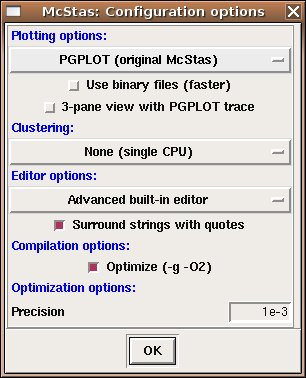
\includegraphics[width=0.3\textwidth]{figures/choose_backend}
  \end{center}
\caption{The ``configuration options'' dialog in \texttt{mcgui}.}
\label{fig:mcgui-choose}
\end{figure}


\noindent The \textbf{Neutron Site} menu contains a list of template/example
instruments as found in the \MCS library, sorted by neutron site. When
selecting one of these, a local copy of the instrument description is
transferred to the active directory (so that users have modification rights) and
loaded. One may then view its source (Edit) and use it directly for
simulations/trace (3D View).
\\\ \\

\noindent The \textbf{Tools} menu gathers minor tools.
\begin{description}
\item[Tools/Plot current/other results] Plot current simulation results and
  other results.
\item[Tools/Online plotting of results] installs a DSA key to be used for ssh
  clustering and MPI (see Section \ref{s:run-mpi}).
\item[Tools/Dataset convert/merge] Opens a GUI to the \verb+mcformat+ tool, in
  order to convert datasets to other formats, merge scattered dataset (e.g. from
  successive or grid simulations), and assemble scan sets. This tool does not
  handle raw event files.
\item[Tools/Shortcut keys] displays the shortcut keys used for running and
  editing instruments.
\item[Tools/Install DSA key] installs a DSA key to be used for ssh clustering
  and MPI (see Section \ref{s:run-mpi}).\index{MPI}\index{Grid computing}
\item[The Histogrammer] In addition to these tools, the
  \verb+Neutron site/Tools/Histogrammer.instr+ example instrument may read
  McStas, Vitess, MCNP and Tripoli event files in order to generate histograms
  of any type.
\end{description}


\noindent The \textbf{Help} menu has the following features, through use of
\verb+mcdoc+ and a web browser. To customize the used web browser, set
the \verb+BROWSER+ environment variable. If \verb+BROWSER+ is not set,
\verb+mcgui+ uses \verb+netscape/mozilla/firefox+ on Unix/Linux and the default browser on
Windows.
\begin{description}
\item[Help/\MCS User manual] calls \verb+mcdoc --manual+, brings up the local
  pdf version of this manual, using a web browser.
\item[Help/\MCS Component manual] calls \verb+mcdoc --comp+, brings up the local
  pdf version of the component manual, using a web browser.
\item[Help/Component library index] displays the component documentation using
  the component \verb+index.html+ index file.
\item[Help/\MCS web page] calls \verb+mcdoc --web+, brings up the \MCS
  website in a web browser.
\item[Help/Tutorial] opens the \MCS tutorial for a quick start.
\item[Help/Current instrument info] generates a description web-page of the
  current edited instrument.
\item[Help/Test \MCS installation] launches a self test procedure to check that
  the \MCS package is installed properly, generates accurate results, and may
  use the plotter to display the results.
\item[Help/Generate component index] (re-)generates locally the component
  \verb+index.html+.
\end{description}


\subsubsection{The run dialog}

\begin{figure}[htb!]
  \begin{center}
    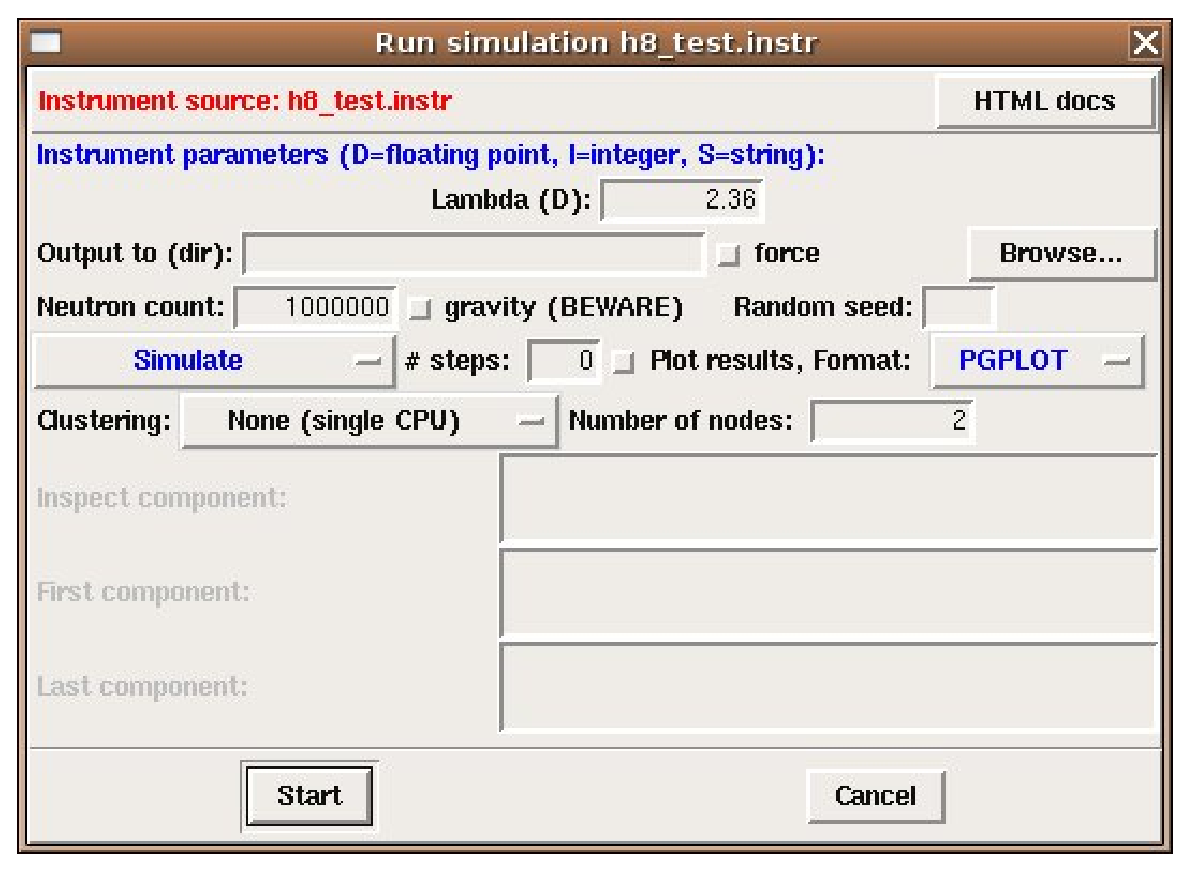
\includegraphics[width=0.45\textwidth]{figures/mcgui-run}
  \end{center}
\caption{The run dialog in \texttt{mcgui}.}
\label{fig:mcgui-run}
\end{figure}
%
The run dialog is used to run simulations. It allows the entry of instrument
parameters as well as the specifications of options for running the simulation
(see section~\ref{s:run-sim} for details). It also allows to run the
\verb+mcdisplay+ (section~\ref{s:mcdisplay}) and \verb+mcplot+
(section~\ref{s:mcplot}) front-ends together with the
simulation.\indexTOOL{mcplot}

The meaning of the different fields is as follows:
\begin{description}
\item[Run:Instrument parameters] allows the setting of the values for the input
  parameters of the instrument. The type of each instrument parameter is given
  in parenthesis after each name. Floating point numbers are denoted by (D) (for
  the C type ``\verb+double+''), (I) denotes integer parameters, and (S) denotes
  strings. For parameter scans and optimizations, enter the minimum and maximum
  values to scan/optimize, separated by a comma, e.g. \verb+1,10+ and do not
  forget to set the \textbf{\# Scanpoints} to more than 1.
\item[Run:Output to] allows the entry of a directory for storage of the
  resulting data files in (like the \verb+--dir+ option). If no name is given,
  the results are stored in the current directory, to be overwritten by the next
  simulation.
\item[Run:Force] Forces McStas to overwrite existing data files
\item[Neutron count] sets the number of neutron rays to
  simulate (the \verb+--ncount+ option).
\item[Run:Gravity] Activates gravitation handling. Not all components full
  support the use of gravitation, but all transport in ``free space'' using the
  PROP\_DT, PROP\_Z0 etc. macros will include propagation with gravity. Only
  local, internal component propagation without the PROP routines will be
  gravity-less. As a conclusion it is considered safe and to high precision
  correct to apply the gravitation setting if one takes care to use the
  Guide\_gravity component and other gravity-supporting guide types in
  combination with non-gravity components that are ``small'' in size,
  i.e. samples, lenses, etc.
\item[Run:Random seed/Set seed to] selects between using a random seed (different
  in each simulation) for the random number generator, or using a fixed
  seed (to reproduce results for debugging).
\item[Run:Simulate/Trace (3D)/Optimize] selects between several modes of
  running the simulation:
  \begin{itemize}
  \item Simulate: perform a normal simulation or a scan when \#steps
    is set to non-zero value
  \item Trace (3D view): View the instrument in 3D tracing individual
    neutrons through the instrument
  \item Optimize: find the optimum value of the simulation parameters
    in the given ranges (see section \ref{s:optimize}).
  \item Backgrounding (bg): Simulate or Optimize in the background.
\end{itemize}
\item[Run:\# steps / \# optim] sets the number of simulation to run when
  performing a parameter scan or the number of iterations to
  perform in optimization mode.
\item[Run:Plot results] -- if checked, the \verb+mcplot+ front-end will be run
  after the simulation has finished, and the plot dialog will appear
  (see below).
\item[Run:Format] quick selection of output format. Binary mode may be checked
  from the ``Simulation/Configuration options'' dialog box.
\item[Run:Clustering method] selects the mechanism to be used for running on
  grids and clusters.  See section~\ref{s:run-mpi} on parallel computing for
  more informations.
\item[Run:Number of nodes] sets the number of nodes to use for MPI/ssh
  clustering.
\item[Run:Inspect component] (Trace mode) will trace only neutron trajectories
  that reach a given component (e.g. sample or detector).
\item[Run:First component] (Trace mode) seletcs the first component to plot
  (default is first) in order to define a region of interest.
\item[Run:Last component] (Trace mode) seletcs the last component to plot
  (default is first) in order to define a region of interest.
\item[Run:Maximize monitor] (Optimization mode) seletcs up to three monitors
  which integral value should be maximized, varying instrument parameters. If no
  monitor is selected, the sum of all monitors is optimized.
\item[Run:Start] runs the simulation.
\item[Run:Cancel] aborts the dialog.
\end{description}
Most of the settings on the run dialog can be saved for your next
\MCS run using 'Save configuration' in the File menu.

Before running the simulation, the instrument definition is automatically
compiled if it is newer than the generated C file (or if the C file is newer
than the executable). The executable is assumed to have a \verb+.out+ suffix in
the filename. NB: If components are changed, automatic compilation is \emph{not}
performed. Instead, use the File/Compile menu item in mcgui.



\subsubsection{The editor window}

The editor window provides a simple editor for creating and modifying instrument
definitions. Apart from the usual editor functions, the ``Insert'' menu provides
some functions that aid in the construction of the instrument definitions:
\begin{description}
\item[Editor Insert/Instrument template] inserts the text for a simple instrument
  skeleton in the editor window.
\item[Editor Insert/Component\ldots] opens up a dialog window with a list of all
  the components available for use in McStas. Selecting a component will
  display a description. Double-clicking will open up a dialog window
  allowing the entry of the values of all the parameters for the
  component (figure~\ref{f:comp_dialog}). See section~\ref{s:instrdefs}
  for details of the meaning of the different fields.

  The dialog will also pick up those of the users own components that are
  present in the current directory when \verb+mcgui+ is started. See
  section~\ref{s:mcdoc} for how to write components to integrate well with this
  facility.
\item[Editor Insert/\textit{Type}] These menu entries give quick access to the
  entry dialog for the various component types available, i.e. Sources, Optics,
  Samples, Monitors, Misc, Contrib and Obsolete.
\end{description}
\begin{figure}[tbp]
  \begin{center}
    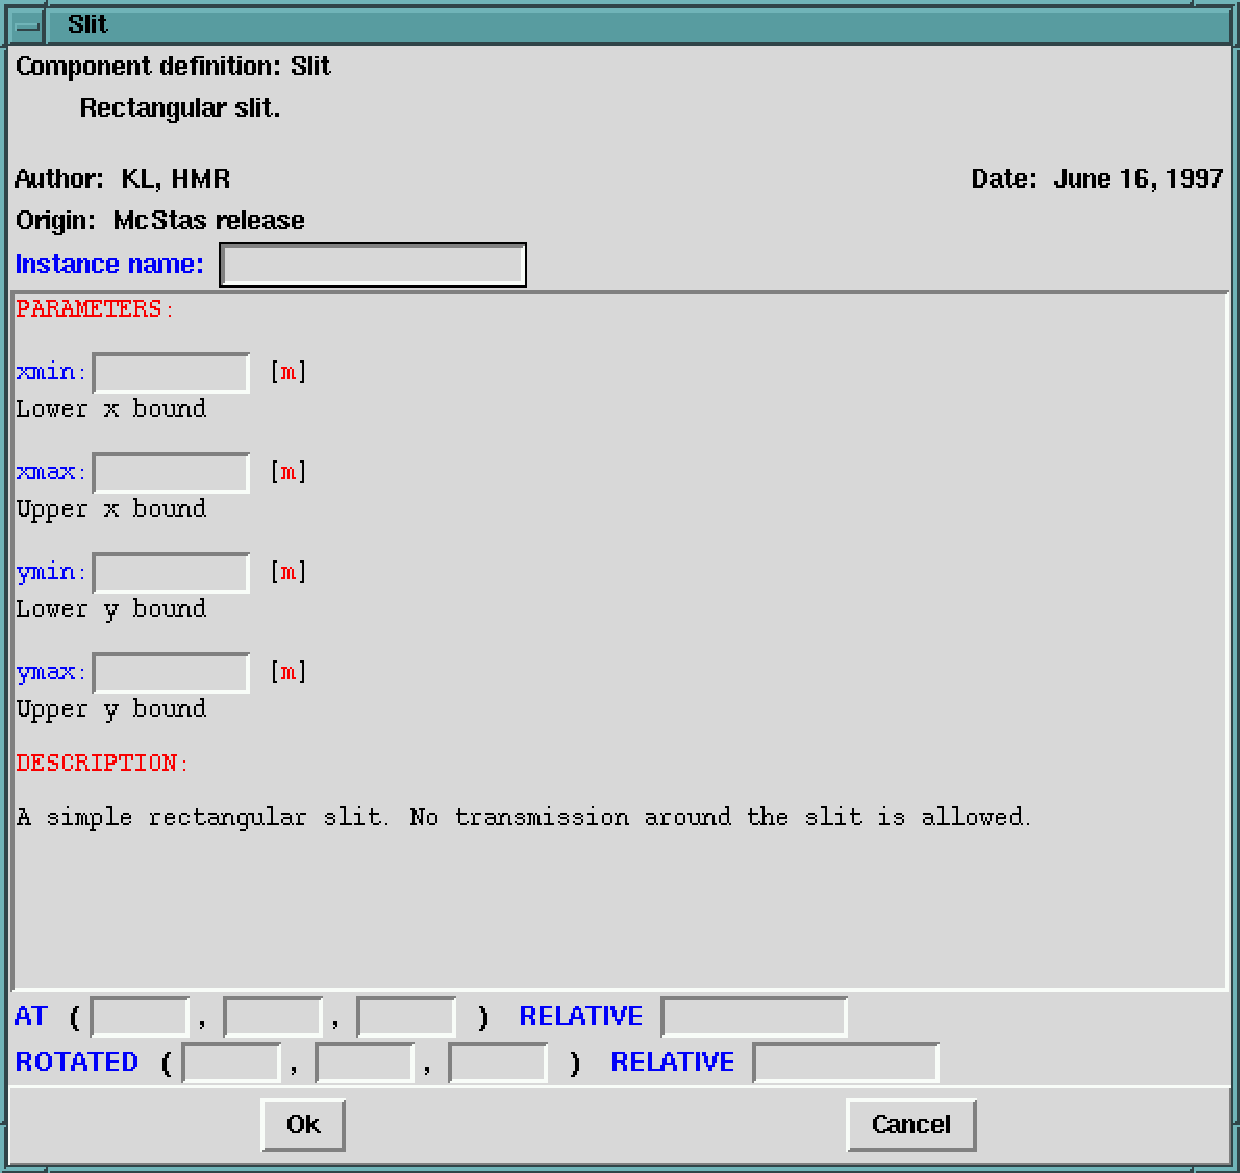
\includegraphics[width=0.55\textwidth]{figures/comp_dialog}
    \caption{Component parameter entry dialog.}
    \label{f:comp_dialog}
  \end{center}
\end{figure}


%-------------------------------------------------------------------------------
\subsection{Running simulations on the commandline (mcrun)}
\label{s:mcrun}
\indexTOOL{mcrun|textbf}
\index{Parameters!instruments}
\index{Parameters!scans}
\index{Parameters!optimization}

The \verb+mcrun+ front-end (mcrun.pl on Windows) provides a convenient
command-line interface for running simulations with the same automatic
compilation features available in the \verb+mcgui+ front-end. It also provides a
facility for running a series of simulations while varying an input parameter.

The command

\begin{bash}
mcrun sim args ...
\end{bash}

will compile the instrument definition \texttt{\textit{sim}.instr} (if
necessary) into an executable simulation \texttt{\textit{sim}.out}. It
will then run \texttt{\textit{sim}.out}, passing the argument list \textit{
  args}

The possible arguments are the same as those accepted by the simulations
themselves as described in section~\ref{s:run-sim}, with the following
extensions:
\begin{itemize}
\item The \verb+-c+ or \verb+--force-compile+ option may be used to force the
  recompilation of the instrument definition, regardless of file dates. This may
  be needed in case any component definitions are changed (in which case
  \verb+mcrun+ does not automatically recompile), or if a new version of McStas
  has been installed.
\item The \texttt{-p \textit{file}} or \texttt{--param=\textit{file}} option may be
  used to specify a file containing assignment of values to the input parameters
  of the instrument definition. The file should consist of specifications of the
  form \texttt{\textit{name\/}=\textit{value\/}} separated by spaces or line
  breaks. Multiple \verb+-p+ options may be given together with direct parameter
  specifications on the command line. If a parameter is assigned multiple times,
  later assignments override previous ones.
\item The \texttt{-N \textit{count}} or \texttt{--numpoints=\textit{count}} option
  may be used to perform a series of \textit{count\/} simulations while
  varying one or more parameters within specified intervals. Such a
  series of simulations is called a \emph{scan}. To specify
  an interval for a parameter \textit{X}, it should be assigned two
  values separated by a comma. For example, the command
\begin{bash}
mcrun sim.instr -N4 X=2,8 Y=1
\end{bash}
would run the simulation defined in \verb+sim.instr+ four times, with
\textit{X} having the values 2, 4, 6, and 8, respectively.

After running the simulation, the results will be written to the file
\verb+mcstas.dat+ by default. This file contains one line for each simulation
run giving the values of the scanned input variables along with the integrated
intensity and estimated error in all monitors. Additionally, a file
\verb+mcstas.m+ (when using Matlab format) is written that can be read by the
\verb+mcplot+ front-end to plot the results on the screen or in a Postscript
file, see section~\ref{s:mcplot}. \indexTOOL{mcplot}
\item When performing a scan, the \texttt{-f \textit{file}} and
  \texttt{--file=\textit{file}} options make \verb+mcrun+ write the output
  to the files \texttt{\textit{file\/}.dat} and \texttt{\textit{file\/}.sim}
  instead of the default names.
\item When performing a scan, the \texttt{-d \textit{dir}} and
  \texttt{--dir=\textit{dir}} options make \verb+mcrun+ put all output in a
  newly created directory \textit{dir}. Additionally, the directory will
  have subdirectories \verb+1+, \verb+2+, \verb+3+,\ldots containing all
  data files output from the different simulations. When the \verb+-d+
  option is not used, no data files are written from the individual
  simulations (in order to save disk space).
\item The \verb+mcrun --test+ command will test your \MCS installation,
  accuracy and plotter. \index{Installing}
\end{itemize}

The \verb+-h+ option will list valid options. The \verb+mcrun+ front-end
requires a working installation of Perl to run.


%-------------------------------------------------------------------------------
\subsection{Graphical display of simulations (mcdisplay)}
\label{s:mcdisplay}
\indexTOOL{mcdisplay|textbf}

The front-end \verb+mcdisplay+ (mcdisplay.pl on Windows) is a graphical
visualization tool, very useful for debugging.  It presents a schematic drawing
of the instrument definition, showing the position of the components and the
paths of the simulated neutrons through the instrument. It is thus very useful
for debugging a simulation, for example to spot components in the wrong position
or to find out where neutrons are getting lost.  (See figures
\ref{fig:mcdisp_PGPLOT}-\ref{fig:mcdisp_Matlab}.)

To use the \verb+mcdisplay+ front-end with a simulation, run it as
follows:
\begin{bash}
mcdisplay sim args ...
\end{bash}

where \verb+sim+ is the name of either the instrument source
\texttt{\textit{sim}.instr} or the simulation program \texttt{\textit{sim}.out} generated with
\MCS, and \textit{args \ldots} are the normal command line arguments for the
simulation, as explained above. The \verb+-h+ option will list valid options.

\indexTOOL{PGPLOT}
\indexTOOL{Matlab}
\indexTOOL{VRML/OpenGL}
\index{OpenGL}
The drawing back-end program may be selected among
PGPLOT, VRML, and Matlab using the -p\textit{PLOTTER} option. For instance, calling
\begin{bash}
mcdisplay --pMatlab ./Samples_vanadium.out ROT=90+
\end{bash}
will output graphics using Matlab.
The \verb+mcdisplay+ front-end can also be run from the \verb+mcgui+ front-end.
\indexTOOL{mcgui}
Examples of plotter appearence for \verb+mcdisplay+ is shown in figures
 \ref{fig:mcdisp_PGPLOT}-\ref{fig:mcdisp_Matlab}.

\paragraph{\MCS /PGPLOT back-end}

This will view the instrument from above. A multi-display that shows the
instrument from three directions simultaneously can be shown using the
\verb+--multi+ option:
\begin{lstlisting}
mcdisplay --multi sim.out args ...
\end{lstlisting}

Click the left mouse button in the graphics window or hit the space key to see
the display of successive neutron trajectories. The `P' key saves a postscript
file containing the current display that can be sent to the printer to obtain a
hardcopy; the `C' key produces color postscript.  To stop the simulation
prematurely, type `Q' or use control-C as normal in the window in which
\verb+mcdisplay+ was started.

To see details in the instrument, it is possible to zoom in on a part of the
instrument using the middle mouse button (or the `Z' key on systems with a one-
or two-button mouse). The right mouse button (or the `X' key) resets the
zoom. Note that after zooming, the aspect ratio of the plot may have changed,
and thus the angles as seen on the display may not match the actual angles.

Another way to see details while maintaining an overview of the instrument is to
use the \verb+--zoom=+\textit{factor} option. This magnifies the display of each
component along the selected axis only, {\em e.g.} a Soller collimator is
magnified perpendicular to the neutron beam but not along it. This option may
produce rather strange visual effects as the neutron passes between components
with different coordinate magnifications, but it is occasionally useful.

When debugging, it is often the case that one is interested only in neutrons
that reach a particular component in the instrument. For example, if there is a
problem with the sample one may prefer not to see the neutrons that are absorbed
in the monochromator shielding. For these cases, the
\verb+--inspect=+\textit{comp\/} option is useful. With this option, only
neutrons that reach the component named \textit{comp\/} are shown in the
graphics display.

As of \MCS 1.10, the PGPLOT version has a special mode for time of flight
applications. Using the new commandline options \verb+--TOF/-T+ and
\verb+--tmax=TMAX+, chopper acceptance diagrams can be generated from the
statistical information from the simulated neutron rays. As the use in
non-interactive, please use with a limited number of neutron rays
(\verb+-n/--ncount+). For export of graphics, combine with e.g. \verb+--gif+.

\indexTOOL{PGPLOT}
The \verb+mcdisplay+ front-end will then require the Perl,
the PGPLOT, and the PGPerl packages to be installed. It may be necessary to set
the \verb+PGPLOT_DIR+ and \verb+PGPLOT_DEV+ environment variable; consult the
documentation for PGPLOT on the local system in case of difficulty.
\indexEV{PGPLOT\_DEV}
\indexEV{PGPLOT\_DIR}
\index{Perl!libraries}

\paragraph{Matlab and back-end}

A 3D view of the instrument, and various operations (zoom, export, print, trace
neutrons, \ldots) is available from dedicated Graphical User Interfaces.  The
\verb+--inspect+ option may be used (see previous paragraph), as well as the
\verb+--first+ and \verb+--last+ options to specify a region of interest.

The \verb+mcdisplay+ front-end will then require the Perl, and
Matlab to be installed. \indexTOOL{Matlab}

\paragraph{VRML/OpenGL back-ends}

When using the \verb+-pVRML+ option, the instrument is shown in Virtual Reality
(using OpenGL). You may then walk aside instrument, or go inside elements
following neutron trajectories. As all neutron trajectories are stored into a
VRML file, you better limit the number of stored trajectories below 1000,
otherwise file size and processing time becomes significant. The
\verb+--inspect+ option is not available in VRML format display.

%-------------------------------------------------------------------------------
\subsection{Plotting the results of a simulation (mcplot)}
\label{s:mcplot}
\indexTOOL{mcplot|textbf}

The front-end \verb+mcplot+ (mcplot.pl on Windows) is a program that produces
plots of all the monitors in a simulation, and it is thus useful to get
a quick overview of the simulation results.

In the simplest case, the front-end is run simply by typing
\begin{bash}
    mcplot
\end{bash}
This will plot any simulation data stored in the current directory, which is
where simulations store their results by default. If the \verb+--dir+ or
\verb+--file+ options have been used (see section~\ref{s:run-sim}), the name of
the file or directory should be passed to mcplot, {\em e.g.} ``\texttt{mcplot
  \textit{dir}}'' or ``\texttt{mcplot \textit{file}}''.  It is also possible to plot
one single text (not binary) data file from a given monitor, passing its name to
mcplot.

The drawing back-end program may be selected among PGPLOT, Matlab, and
Gnuplot using either the -p\textit{PLOTTER} option (e.g. \texttt{mcplot -pMatlab
file}) or using the current \verb+MCSTAS_FORMAT+ environment
variable.
\indexEV{MCSTAS\_FORMAT}

Except for the NeXus format, all other plotters read the legacy 
McStas/PGPLOT text based data format. 

The \verb+mcformat+ utility will convert any \MCS
result into an other data format (see section \ref{s:mcformat}), but restricting to text
data sets. In this case, we recommend to generate data sets using PGPLOT/McStas
format, and translate into any other format using \verb+mcformat+.

The \verb+mcplot+ front-end can also be run from the \verb+mcgui+ front-end.
\indexTOOL{mcgui}

The initial display shows plots for each detector in the simulation.
Examples of plotter appearence for \verb+mcplot+ is shown in figures
 \ref{fig:mcdisp_PGPLOT}-\ref{fig:mcplot_figs}.

\paragraph{\MCS /PGPLOT back-end}
\indexTOOL{PGPLOT}
Clicking the left mouse button on a plot produces a full-window version
of that plot. The `P' key saves a postscript file containing the current
plot that can be sent to the printer to obtain a hardcopy; the `C' key
produces color postscript.
The `Q' key quits the program (or CTRL-C in the controlling
terminal may be used as normal).

To use the \verb+mcplot+ front-end with PGPLOT, the programs Perl, PGPLOT,
PgPerl, and PDL must all be properly installed on the system.  It may be
necessary to set the \verb+PGPLOT_DIR+ and \verb+PGPLOT_DEV+ environment
variable; consult the documentation for PGPLOT on the local system in case of
difficulty.
\indexEV{PGPLOT\_DEV}
\indexEV{PGPLOT\_DIR}
\index{Perl!libraries}

\paragraph{Matlab back-end}

A dedicated \MCS /Mcplot Dialog or menu attached to the plotting window is
available, and provides many operations (duplication, export, colormaps,
\ldots).  The corresponding 'mcplot' Matlab function may be called
from these language prompt with the same method as in section~\ref{s:run-sim},
e.g:
\begin{matlab}
    matlab> s=mcplot;
    matlab> help mcplot
    matlab> s=mcplot('mcstas.m');
    matlab> mcplot(s);
\end{matlab} \indexTOOL{Matlab}

A full parameter scan simulation result, or simply one of its scan steps may be
displayed using the 'Scan step' menu item.  When the \verb|+nw| option is
specified, a separate Matlab window will appear (instead of being
launched in the current terminal). This will then enable Java support under
Matlab, resulting in additional menus and tools. On
the other hand, the \verb|-nw| option will force Matlab to run in the
current terminal, which is usually faster.

To use the \verb+mcplot+ front-end, the programs Perl, and
Matlab are required. \indexTOOL{Matlab}


%-------------------------------------------------------------------------------
\subsection{Plotting resolution functions (mcresplot)}
\label{s:mcresplot}
\indexTOOL{mcresplot|textbf}
\indexTOOL{PGPLOT}

\begin{figure}[tb!]
  \begin{center}
    \includegraphics[angle=-90,width=0.97\textwidth]{figures/mcresplot_PGPLOT.ps}
  \end{center}
\caption{Output from \texttt{mcresplot} with PGPLOT backend.
  Use P, C and G keys to write hardcopy files.}
\label{fig:mcresplot_PGPLOT}
\end{figure}

The \verb+mcresplot+ front-end is used to plot the resolution function,
particularly for triple-axis
%or inverse geometry time-of-flight
spectrometers, as calculated by the Res\_sample component or TOF\_res\_sample
for time-of-flight instruments. It requires to have a Res\_monitor component
further in the instrument description (at the detector position).
%(see section~\ref{s:res_sample}).
This front-end
has been included in the release since it may be useful
despite its somewhat rough user interface.

The \verb+mcresplot+ front-end is launched with the command
\begin{lstlisting}
mcresplot outfile
\end{lstlisting}
Here, \textit{outfile\/} is the name of a file output from a simulation using
the Res\_monitor component.
% (section~\ref{s:res_monitor}).

This front-end currently only works with the PGPLOT plotter, but port for
Matlab may be written in the future.

The front-end will open a window displaying projections of the 4-dimensional
resolution function $R(\boldsymbol{Q}, \omega)$, measured at a
particular choice of $\boldsymbol{Q}$ and $\omega$, see the component
manual. The covariance matrix of the
resolution function, the resolution along each projection axis and the resulting
resolution matrix are also shown, as well as the instrument name and parameters
used for the simulation.

To use the \verb+mcresplot+ front-end, the programs Perl, PGPLOT, PgPerl,
and PDL must all be properly installed on the system.
\index{Perl!libraries}

%-------------------------------------------------------------------------------
\subsection{Creating and viewing the library, component/instrument help and
  Manuals (mcdoc)}
\label{s:mcdoc-run}
\indexTOOL{mcdoc|textbf}

\MCS provides an easy way to generate automatically an HTML help page about a
given component or instrument, or the whole \MCS
library. \index{Library!Components}
\begin{lstlisting}
mcdoc
mcdoc {comp|instr}
mcdoc --tools
\end{lstlisting}
The first example generates an \textit{index.html} catalog file using the available
components and instruments (both locally, and in the \MCS library). The library
catalog of components is opened using the \verb+BROWSER+ environment variable
\indexEV{BROWSER}
(e.g. netscape, konqueror, nautilus, MSIE,
mozilla, \ldots). If the \verb+BROWSER+ is not defined, the help is displayed as
text in the current terminal. This latter output may be forced with the
\verb+-t+ or \verb+--text+ option.

Alternatively, if a component or instrument \textit{comp} is specified as in the
second example, it will be searched within the library, and an HTML help will be
created for all available components matching \textit{comp}.

The last example will list the name and description of all \MCS tools.

Additionally, the options \verb+--web+, \verb+--manual+ and \verb+--comp+ will
open the \MCS web site page, the User Manual (this document) and the Component
Manual, all requiring \verb+BROWSER+ to be defined. Finally, the \verb+--help+
option will display the command help, as usual.

See section~\ref{s:mcdoc} for more details about the McDoc usage and header
format.  To use the \verb+mcdoc+ front-end, the program Perl should be
available.

%-------------------------------------------------------------------------------
\subsection{Translating \MCS components for Vitess (mcstas2vitess)}
\label{s:mcstas2vitess}
\indexTOOL{mcstas2vitess|textbf}
\index{Library!vitess-lib}
\index{Vitess!vitess-lib}

Any \MCS component may be translated for usage with Vitess (starting from
Vitess version 2.3). The syntax is simply \index{Library!components}
\begin{lstlisting}
mcstas2vitess Compo.comp
\end{lstlisting}
This will create a Vitess module of the given component.

Let us assume the component \verb+Compo+ shall be translated. The tool first
creates a small instrument called \verb+McStas_Compo.instr+ consisting of
\begin{enumerate}
\item component Vitess\_input
\item component \verb+Compo+
\item component Vitess\_output
\end{enumerate}

This file is parsed to generate the C file \verb+McStas_Compo.c+. The last step
is to compile the C-file and build the executable Vitess module
\verb'McStas_compo'. For both steps \MCS is used as for any other
instrument. \verb'McStas_compo' has to be moved to the directory 'MODULES' that
contains all VITESS executables.

Additionally, a file \verb'McStas_compo.tcl' is created that contains (most of)
what is needed to get a GUI window in VITESS. To obtain that, the content of
this file has to added into 'vitess.tcl'. To make it accessible within the given
GUI structure of VITESS, it is necessary to add the name 'compo' - NO capital
letters ! - to one of the folders in 'proc makeModuleSets{}' (beginning of
'vitess.tcl').

The component Virtual\_input transfers all neutron parameters to the \MCS
definition of the co-ordinate system and the units used. (Of course
Virtual\_output transfers it back.) This means that 'Compo' works with the
McStas definition of co-ordinate system and units, while it is used as a VITESS
module. Be careful with axis labeling.

The original parameters of the component and its position have to be given. The
origin of this shift is the center of the end of the previous module, (as it is
always the case in VITESS).

It is important to notice that, as VITESS uses the standard output stream
(\verb+stdout+) to send neutron events, all information printed to screen must
use the \emph{error} stream \verb+stderr+, so that \emph{all} \verb+printf(...)+
and \verb+fprintf(stdout, ...)+ occurrences should be changed manually into
\verb+fprintf(stderr, ...)+.

To use the \verb+mcstas2vitess+ front-end, the program Perl should be available.

%-------------------------------------------------------------------------------
\subsection{Translating and merging \MCS results files (all text formats)}
\label{s:mcformat}
\indexTOOL{mcformat|textbf}
\indexTOOL{Matlab}
\index{Data formats}
\index{Grid computing}

If you have been running a \MCS simulation with a given text format output, but
finally plan to look at the results with an other plotter (e.g. you ran a
simulation with PGPLOT output and want to view it using Matlab), you may use
% FIXME syntax check!
\begin{lstlisting}
mcformat {file|dir} -d target_dir --format=TARGET_FORMAT
\end{lstlisting}
to translate files into format TARGET\_FORMAT (e.g. NeXus). When given a directory, the
translation works recursively. The conversion works only for text files.

The \verb+--merge+ option may be used to merge similar files, e.g. obtained from
grid systems, just as if a longer run was achieved.

The \verb+--scan+ option may be used to reconstruct the scan data from a set of
directories which vary by instrument parameters. For instance, you ran a scan,
but finally realized you should have prolonged it. Then simply simulate the
missing bits, and apply
\verb+mcformat -d scan_data --format=PGPLOT --scan step0 .. stepN+. The
resulting scan data is compatible with \verb+mcplot+ only when generating
PGPLOT/McStas format.\indexTOOL{mcplot}
You may conjugate this option with the
\verb+--merge+ in order to add/merge similar data sets before re-building the
scan.

The data files are analyzed by searching keywords inside data files
(e.g. 'Source' for the source instrument description file). If some file names or
component names match these keywords (e.g. using a file 'Source.psd'), the
extracted metadata information may be wrong, even though the data itself will be
correct.\index{Bugs!wrong metadata in translating and merging results files}

%%%%%%%%%%%%%%%%%%%%%%%%%%%%%%%%%%%%%%%%%%%%%%%%%%%%%%%%%%%%%%%%%%%%%%%%%%%%%%%%
\section{Data formats - Analyzing and visualizing the simulation results}
\label{s:analyze}
\index{Data formats}

To analyze simulation results, one uses the same tools as for analyzing
experimental data, \textit{i.e}. programs such as Matlab, NumPy, IDL.  The
output files from simulations are usually simple text files containing headers
and data blocks. If data blocks are empty they may be accessed referring to an
external file indicated in the header.

Each data file contains information about the simulation, the instrument, the
parameters used, and of course the signal, the estimated error on the signal,
and the number of events used in each bin. Additionally, all data files indicate
their first moment (mean value) and second moment (half width) in the
'statistics' field.

The available data formats are the legacy McStas (McCode) format, and the HDF/NeXus binary when the needed libraries are installed.
\indexEV{MCSTAS\_FORMAT}

In order for the user to choose the data format, we recommend to set it using
the \verb+--format=FORMAT+ or alternatively \textit{via} the MCSTAS\_FORMAT
environment variable, which will also make the front-end programs able to import
and plot data and instrument consistently (see Section \ref{s:run-sim}). 

Note that the neutron event counts in detectors are typically not very
meaningful except as a way to measure the performance of the
simulation. Use the simulated intensity instead whenever analyzing
simulation data.

%-------------------------------------------------------------------------------
\subsection{\MCS and PGPLOT format}
\indexTOOL{PGPLOT!format}
\index{Data formats}
The \MCS original format, which is
equivalent to the PGPLOT format, is simply columns of ASCII text that most
programs should be able to read.

One-dimensional histogram monitors (time-of-flight, energy)
write one line for each histogram bin. Each line contains a number
identifying the bin (\textit{i.e}.\ the time-of-flight) followed by
three numbers: the simulated intensity, an estimate of the statistical
error as explained in section~\ref{s:staterror}, and the number of
neutron events for this bin.

Two-dimensional histogram monitors (position sensitive detectors) output $M$
lines of $N$ numbers representing neutron intensities, where $M$ and $N$ are the
number of bins in the two dimensions. The two-dimensional monitors also store
the error estimates and event counts as additional matrices.

Single-point monitors output the neutron intensity, the estimated
error, and the neutron event count as numbers on the
terminal. (The results from a series of simulations may be combined in a
data file using the \verb+mcrun+ front-end as explained in
section~\ref{s:mcrun}).

When using one- and two-dimensional monitors, the integrated intensities are
written to terminal as for the single-point monitor type, supplementing file
output of the full one- or two-dimensional intensity distribution. Both one- and
two-dimensional monitor output by default start with a header of comment lines,
all beginning with the `\verb+#+' character.  This header gives such information
as the name of the instrument used in the simulation, the values of any
instrument parameters, the name of the monitor component for this data file,
\textit{etc}. The headers may be disabled using the \verb+--data-only+ option in
case the file must be read by a program that cannot handle the headers.

In addition to the files written for each one- and two-dimensional monitor
component, another file (by default named \verb+mcstas.sim+) is also
created. This file is in a special \MCS ASCII format. It contains all available
information about the instrument definition used for the simulation, the
parameters and options used to run the simulation, and the monitor components
present in the instrument. It is read by the \verb+mcplot+ front-end (see
section~\ref{s:mcplot}). This file stores the results from single monitors, but
by default contains only pointers (in the form of file names) to data for one-
and two-dimensional monitors. By storing data in separate files, reading the
data with programs that do not know the special \MCS file format is
simplified. The \verb+--file+ option may be used to store all data inside the
\verb+mcstas.sim+ file instead of in separate files.

%-------------------------------------------------------------------------------
\subsection{NeXus format}
\indexTOOL{NeXus}
\index{HDF5|see{NeXus format}}
\index{Data formats}
\label{r:nexus}

The NeXus format~\cite{nexus_webpage} is a platform independent HDF binary data
file. To have \MCS use it
\begin{enumerate}
\item the HDF and NeXus libraries must have been installed (libNeXus and headers)
\item the compilation of instruments must be done with the
  \verb+-DUSE_NEXUS -lNeXus+ flag (see Section \ref{s:nexus}). This is
  automated with the \verb+mcrun+ tool (Section \ref{s:mcrun}).
\end{enumerate}
All results are saved in a single file, containing 'groups' of data. To view
such files, install and use HDFView (or alternatively HDFExplorer). This Java
viewer can show content of all detectors, including metadata (attributes). Basic
detector images may also be generated.

%%%%%%%%%%%%%%%%%%%%%%%%%%%%%%%%%%%%%%%%%%%%%%%%%%%%%%%%%%%%%%%%%%%%%%%%%%%%%%%%
\section{Using computer Grids and Clusters}
\label{s:run-mpi}
\index{Parallel computing|textbf}
\index{MPI|textbf}
\index{Grid computing|textbf}
\index{mcstas-hosts}

Parallelizing a computation is in general possible when dependencies between
  each computation are not too strong. The situation of \MCS is
  ideal since each neutron ray can be simulated without interfering with
  other simulated neutron rays. Therefore each neutron ray can be simulated
  independently on a set of computers.

  When computing $N$ neutron rays with $p$ computers, each computer will
  simulate $\frac{N}{p}$ neutrons. As a result there will be $p \cdot
  \frac{N}{p} = N$ neutrons simulated. As a result, \MCS generates two kinds of
  data sets:
\begin{itemize}
\item intensity measurements, internally represented by three
  values $(p_0, p_1, p_2)$ where $p_0$, $p_1$, $p_2$ are
  additive. Therefore the final value of $p_0$ is the sum of all
  local value of  $p_0$ computed on each node. The same rule applies
  for $p_1$ and $p_2$. The evaluation of the intensity errors $\sigma$
  is performed using the final $p_0$, $p_1$, and $p_2$ arrays (see Section \ref{s:staterror}).
\item event lists: the merge of events is done by concatenation
\end{itemize}

\MCS provides three methods in order to distribute computations on many
computers.
\begin{itemize}
\item when using a set of nodes (grid, cluster or multi-cores), it is possible
  to distribute simulations on a list of computers and multi-core machines (see
  section \ref{s:ssh-grid}). Results are automatically merged after completion.
  This method is very efficient, and only requires SSH server to be
  installed/configured on slave machines.  In order to use an heterogeneous
  system, a C compiler should be optionally installed on slave machines.
\item when using an homogeneous computer cluster, each simulation (including
  scan steps) may be computed in parallel using MPI. We recommend this method on
  clusters (see section \ref{s:mpi}).
\end{itemize}

Last but not least, you may run simulations manually on a number of machines.
Once the distributed simulation have been completed, you may merge their results
using \verb+mcformat+ (see section \ref{s:mcformat})
\indexTOOL{mcformat}
in order to obtain a set of files just as if it had been executed on a single
machine.

All of these methods can be used, when available, from \texttt{mcgui}.

%-------------------------------------------------------------------------------
\subsection{Distribute mcrun simulations on grids, multi-cores and clusters (SSH
  grid)}
\label{s:ssh-grid}
This method distributes simulations on a set of machines using \emph{ssh}
connections, using a command such as \verb+mcrun --grid=4 ...+.  Each of the
scan steps is split and executed on distant slave machines, sending the
executable with \emph{scp}, executing single simulations, and then retrieving
individual results on the master machine. These are then merged using
\texttt{mcformat}.

The \verb'mcrun' script has been adapted to use transparently SSH grids. The
syntax is:
\begin{itemize}
\item \verb'--grid=<number>': tells \verb'mcrun' to use the grid over \verb'<number>' nodes.
\item \verb'--machines=<file>': defines a text file where the nodes which are to
  be used for parallel computation are listed; by default, \verb'mcrun' will
  look at \verb'$HOME/.mcstas-hosts' and
  \verb'MCSTAS/tools/perl/mcstas-hosts'. When used on a single SMP machine
  (multi-core/cpu), this option may be omitted.
\item \verb'--force-compile': this option is required on heterogeneous systems.
  The C code is sent to all slaves and simulation is compiled on each node
  before starting computation. The default is to send directly the executable
  from the master node, which only works on homogeneous systems.  computation.
\end{itemize}

This method shows similar efficiency as MPI, but without MPI installation. It is
especially suited on multi-core machines, but may also be used on any set of
distant machines (grids), as well as clusters. For Windows master machines, we
recommend the installation of the PuTTY SSH client. The overhead is proportional
to the number of nodes and the amount of data files to transfer per
simulation. It is usually larger than the pure MPI method. We thus recommend to
launch long runs on fewer nodes rather than many short runs on many nodes.

\subsubsection{Requirements and limitation (SSH grids)}

  \begin{enumerate}
  \item{A master machine with an SSH client, and \MCS installation.}
  \item{A set of machines (homogeneous or heterogeneous) with SSH servers.}
  \item{On heterogeneous grids, a C compiler must also be installed on all slave
      nodes.}
  \item{\texttt{ssh} access from the master node (where \MCS is
      installed) to the slaves through e.g. DSA keys \emph{without} a
      password. These keys should be generated using the command
      \texttt{ssh-keygen}. Run \emph{e.g.} \texttt{ssh-keygen -t dsa} on
      master node, enter no passphrase and add resulting
      \texttt{.ssh/id\_dsa.pub} to \texttt{.ssh/authorized\_keys}
      on all the slave nodes. The key generation and registering mechanism
      may be done automatically for the local machine from the
      \emph{Help menu/Install DSA key} item of \verb+mcgui+.}
  \item{The machine names listed in the file \texttt{.mcstas-hosts} in
      your home directory or in the \texttt{MCSTAS/tools/perl/mcstas-hosts} on
      the master node, one node per line. The \verb'--machines=<file>' option
      enables to specify the hosts file to use. If it does not exist, only
      the current machine will be used (for multi-processor/core machines).}
  \item{Without ssh keys, passwords will be prompted many times. To avoid this,
      we recommend to use only the local machine (for multi-cores/cpu), i.e. do
      not use a machine hosts file.}
  \item{If your simulation/instrument requires \emph{data files} (Powders, Sqw,
      source description, ...), these must be copied at the same level as the
      instrument definition. They are sent to all slave nodes before starting
      each computation.  Take care to limit as much as possible the required
      data file volume in order to avoid large data transfers.}
  \item Interrupting or sending Signals may fail during computations. However,
  simulation scans can be interrupted as soon as the on-going computation
  step ends.
\item With heterogeneous systems, we recommend to use the
  \verb+mcrun --force-compile+ command rather than McGUI, which may skip the
  required simulation compilation on slaves.
  \end{enumerate}

%-------------------------------------------------------------------------------
\subsection{Parallel computing (MPI)}
\label{s:mpi}
The MPI support requires that MPICH (recommended), or alternatively LAM-MPI or
OpenMPI, is installed on a set of nodes. This usually also requires properly
setup \texttt{ssh} connections and keys as indicated in the ssh grid system
(Section \ref{s:ssh-grid}). Some OpenMPI implementations do not recognize
multi-cores as separate nodes. In this case, you should use MPICH, or the SSH
grid.

There are 3 methods for using MPI
\begin{itemize}
\item Basic usage requires to compile and run the simulation by hand (mpicc, mpirun).
  This should be used when running LAM-MPI.
\item A much simpler way is to use \verb+mcrun -c --mpi=NB_CPU ...+ which will
  recompile and run MPICH.
\item The McGUI interface supports MPICH from within the Run Dialog.
\end{itemize}

The MPI support is especially suited on clusters. As an alternative, the SSH
grid presented above (section \ref{s:ssh-grid}) is very flexible and requires
lighter configuration.

\subsubsection{Requirements and limitation (MPI)}

To use MPI you will need
  \begin{enumerate}
  \item{A master machine with an SSH client/server, and \MCS installation.}
  \item{A set of Unix machines of the same architecture (binary compatible) with
      SSH servers.}
  \item{ \texttt{ssh} access from the master node (where \MCS is
      installed) to the slaves through e.g. DSA keys \emph{without} a
      password. These keys should be generated using the command
      \texttt{ssh-keygen}. Run \emph{e.g.} \texttt{ssh-keygen -t dsa} on
      master node, enter no passphrase and add resulting
      \texttt{.ssh/id\_dsa.pub} to \texttt{.ssh/authorized\_keys}
      on all the slave nodes. The key generation and registering mechanism
      may be done automatically for the local machine from the
      \emph{Help menu/Install DSA key} item of \verb+mcgui+.}
  \item{The machine names listed in the file \texttt{.mcstas-hosts} in
      your home directory or in the \texttt{MCSTAS/tools/perl/mcstas-hosts} on
      the master node, one node per line. The \verb'--machines=<file>' option
      enables to specify the hosts file to use. If it does not exist, only
      the current machine will be used (for multi-processor/core machines).}
  \item{Without ssh keys, passwords will be prompted many times. To avoid this,
      we recommend to use only the local machine (for multi-cores/cpu), i.e. do
      not use a machine hosts file.}
  \item Signals are \emph{not} supported while simulating with MPI (since
    asynchronous events cannot be easily transmitted to all nodes). This
    means it is not possible to cancel an on-going computation. However,
    simulation scans can be interrupted as soon as the on-going computation
    step ends.
  \item MPI must be correctly configured: if using \verb'ssh', you
    have to set ssh keys to avoid use of passwords; if
    using \verb'rsh', you have to set a \verb'.rhosts' file.
    On non-local accounts, this procedure may fail and ssh always require passwords.
  \end{enumerate}

\subsubsection{MPI Basic usage}

To enable parallel computation, compile McStas output C-source file
with \verb'mpicc' with the flag \verb'-DUSE_MPI' and run it using the
wrapper of your MPI implementation (\verb'mpirun' for mpich or lammpi) :
\begin{bash}
  # generate a C-source file [sim.c]
  mcstas sim.instr

  # generate an executable with MPI support [sim.mpi]
  mpicc -DUSE_MPI -o sim.mpi sim.c

  # execute with parallel processing over <N> computers
  # here you have to list the computers you want to use
  # in a file [machines.list] (using mpich implementation)
  # (refer to MPI documentation for a complete description)
  mpirun -machinefile machines.list -n <N> \
         ./sim.mpi <instrument parameters>
  ...
\end{bash}

If you don't want to spread the simulation, run it as usual:
\begin{bash}
  ./sim.mpi <instrument parameters>
\end{bash}

%-------------------------------------------------------------------------------
\subsection{McRun script with MPI support (mpich)}

The \verb'mcrun' script has been adapted to use MPICH implementation
of MPI. Two new options have been added:
\begin{itemize}
\item \verb'--mpi=<number>': tells \verb'mcrun' to use MPI, and to
  spread the simulation over \verb'<number>' nodes
\item \verb'--machines=<file>': defines a text file where the nodes which are to
  be used for parallel computation are listed; by default, \verb'mcrun' will
  look at \verb'$HOME/.mcstas-hosts' and
  \verb'MCSTAS/tools/perl/mcstas-hosts'. When used on a single SMP machine
  (multi-core/cpu), this option may be omitted.
\end{itemize}
When available, the MPI option will show up in the \verb+mcgui+ Run
dialog. Specify the number of nodes required.

Suppose you have four machines named \verb'node1' to \verb'node4'.
A typical machine list file, \verb'machines.list' looks like :
\begin{lstlisting}
node1
node2
node3
node4
\end{lstlisting}

You can then spread a simulation \verb'sim.instr' using \verb'mcrun' :
\begin{bash}
  mcrun -c --mpi=4 --machines=machines.list \
        sim.instr <instrument parameters>
\end{bash}

\begin{paragraph}{Warning:} when using \verb'mcrun' with MPI, be sure to
  recompile your simulation with MPI support (see \verb'-c' flag of
  \verb'mcrun'): a simulation compiled without MPI support cannot be used with
  MPI, whereas a simulation compiled with MPI support can be used without MPI.
\end{paragraph}

%-------------------------------------------------------------------------------
\subsection{McStas/MPI Performance}

Theoretically, a computation which lasts $T$ seconds on a single computer,
should lasts at least $\frac{T}{p}$ seconds when it is distributed over $p$
computers. In practice, there will be overhead time due to the split and merge
operations.
\begin{itemize}
\item the split is immediate: constant time cost ${\cal O}(1)$
\item the merge is at worst linear against the number of computers:
  \begin{itemize}
  \item linear time cost~: ${\cal O}(p)$ when saving an event list
  \item logarithmic time cost: ${\cal O}(\log{p})$ when not saving an
  event list
  \end{itemize}
\end{itemize}

The efficiency of \MCS using MPI has been tested on large clusters, up to 500
nodes.  The computation time decreases in the same proportion as the number of
nodes, showing an ideal efficiency. However, a small overhead may appear
depending on the cluster internal network load, which may be estimated at most
of about 10-20 s.  This overhead comes from the spread and the fusion of the
computations. For instance, spreading a computation implies often an \verb'rsh'
or and \verb'ssh' session to be opened on every node.  To reach the best
efficiency, the computation time should not be lower than 30 seconds, or the
overhead time may become significant compared to total time.

\begin{figure}[htb!]
  \begin{center}
    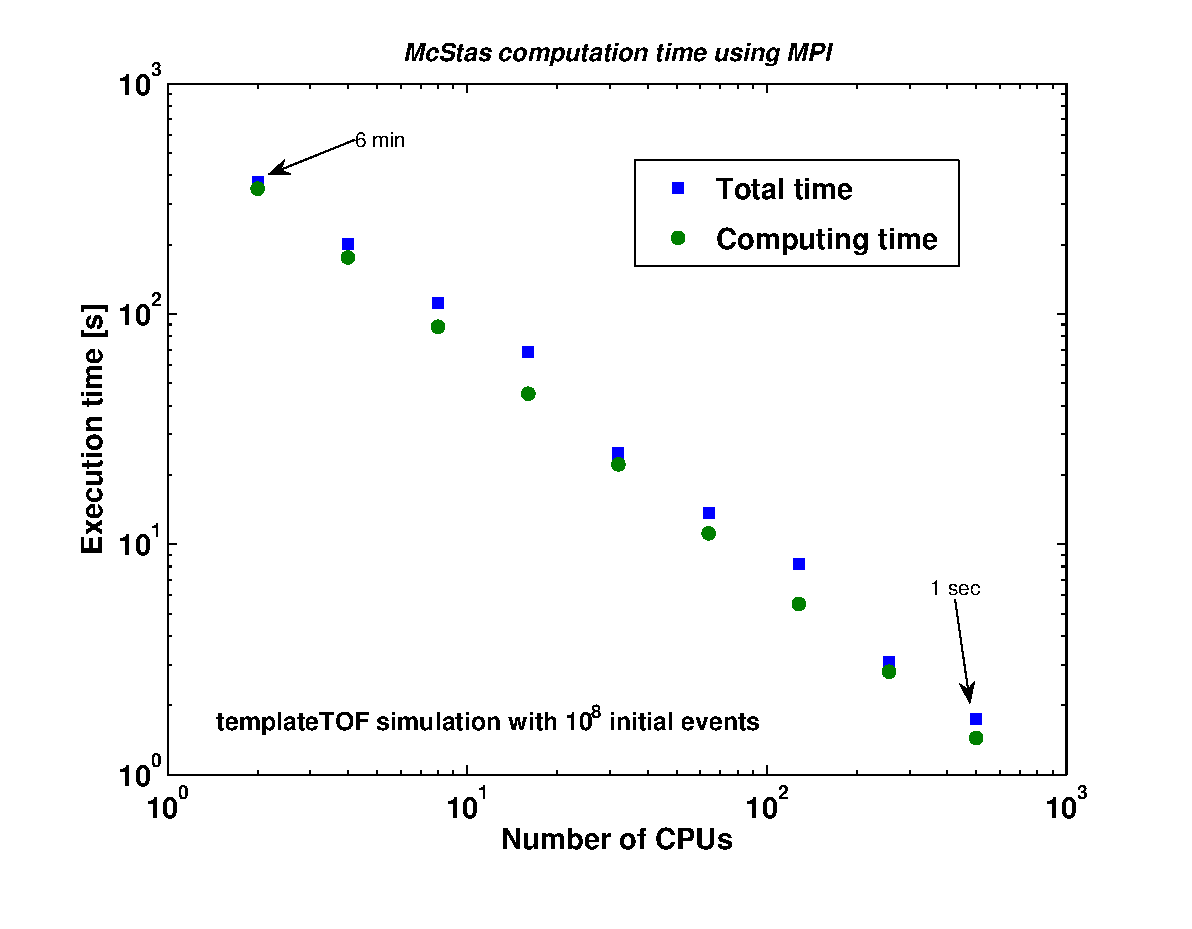
\includegraphics[width=0.55\textwidth]{figures/mpi_efficiency.eps}
  \end{center}
  \caption{McStas/MPI execution time as a function of computing nodes, with
   \textit{templateTOF} instrument and 1e8 initial neutron events. Tests performed on
    Lonestar@TACC (US Teragrid, 2008).}
\label{fig:mpi_efficiency}
\end{figure}

%-------------------------------------------------------------------------------
\subsection{MPI and Grid Bugs and limitations}
\index{Bugs!MPI and grid}

\begin{itemize}
\item Some header of output files might contain minor errors.
\item The computation split does not take into account the speed or the
  load of nodes: the overall time of a distributed computation is
  forced by the slowest node; for optimal performance, the ``cluster''
  should be homogeneous.
\item Interacting with a running simulation (USR1 and USR2 signals) is disabled
  with MPI.
\end{itemize}

%%% Local Variables:
%%% mode: latex
%%% TeX-master: "manual"
%%% End:
